\appendix
\appendixpage
\addappheadtotoc

\setcounter{chapter}{0}

\chapter{Matériels généraux}

\section{Conventions}

\label{sec:conv_fourier}

\subparagraph{}Dans tout cet ouvrage, nous définissons la transformée de Fourier d'une fonction $f(\mathbf{r})$ dans l'espace continu selon la convention :

\begin{equation}
	\hat{f}(\mathbf{q}) = \int \mathrm{d}\mathbf{r}~f(\mathbf{r})e^{-i\mathbf{q}\cdot\mathbf{r}}
\end{equation}

\noindent et de manière réciproque :

\begin{equation}
	f(\mathbf{r}) = \frac{1}{(2\pi)^D}\int \mathrm{d}\mathbf{q}~\hat{f}(\mathbf{q})e^{i\mathbf{q}\cdot\mathbf{r}}
\end{equation}

\noindent avec $D$ la dimension de l'espace. Nous utilisons aussi parfois par ailleurs la notation $\mathcal{F}[\cdot]$ à la place de la notation $\hat{\cdot}$ pour des soucis de lisibilité.

\subparagraph{}Dans le cas de grandeurs discrètes définies sur un réseau, nous utiliserons aussi la notation $\hat{\cdot}$ pour désigner la transformée de Fourier discrète associée. Celle-ci est alors définie selon les conventions choisies par le module cuFFT de CUDA \cite{cuda}. Pour un réseau 1D de taille $L$ dans l'espace réel défini par les positions $x_n = n$ (réseau de pas $1$) on a :

\begin{equation}
	\hat{f}(q_m = \frac{2\pi}{L}m) = \sum_{n} f(x_n)e^{-i q_m x_n}
	\label{eq:TFdisc}
\end{equation}

\section{Implémentation discrète des propagateurs}

\label{sec:impl_disc_propag}

\subparagraph{}Comme nous l'avons relevé dans le \autoref{chapter:yielding}, l'implémentation des propagateurs d'interaction dans l'espace de Fourier discret doit être réalisée d'une certaine manière afin d'obtenir, dans l'espace réel discret, une évolution bien définie (i.e. ne présentant pas d'instabilités numériques, voir \autoref{sec:instab_yielding}). Pour ce faire, entre la forme continue $\hat{\mathcal{G}}(\mathbf{q})$ du propagateur dans l'espace de Fourier et la forme discrète associée $\hat{G}(\mathbf{q}_n)$, une conversion est à réaliser pour l'équivalence entre le nombre d'onde continu $\mathbf{q}$ et le nombre d'onde discret $\mathbf{q}_n$. 

\subparagraph{}Une manière de comprendre cette conversion est de considérer l'exemple simple du propagateur représenté par l'opérateur laplacien $\nabla^2$ en 1D. Dans l'espace continu, on a :

\begin{equation}
	\nabla^2 f(x) \xrightarrow[]{\mathcal{F}} -q^2 \hat{f}(q)
\end{equation}

\noindent Dans l'espace discret représenté par le réseau de positions $\{x_n = n\}$, l'opérateur laplacien est calculé par une méthode de différences finies selon :

\begin{equation}
	\nabla^2 f(x_n) \equiv f(x_{n+1})+f(x_{n-1})-2f(x_n)
\end{equation}

\noindent En appliquant la transformée de Fourier discrète donnée par l'\autoref{eq:TFdisc}, on obtient :

\begin{equation}
	\nabla^2 f(x_n) \xrightarrow[]{\mathcal{F}} [2\cos(q_n)-2]\hat{f}(q_n)
\end{equation}

\noindent Ainsi, pour retrouver l'équivalence entre forme continue et forme discrète dans l'espace de Fourier, la conversion $q^2 \rightarrow 2(1-\cos (q_n))$ est nécessaire. C'est donc selon ce raisonnement que les propagateurs d'interaction sont implémentés numériquement dans les \autoref{chapter:Susp} et \autoref{chapter:yielding}.

\chapter{Annexes au chapitre 1}

\section{Réalisations expérimentales de la transition de dépiégeage}

\label{app:exp_depinning}

\subparagraph{}Dans cette section, nous présentons deux réalisation de la transition de dépiégeage en matière molle.

\paragraph{Dynamique de mouillage à la ligne triple}

\subparagraph{}En condition de mouillage non-total, lorsque l'on dépose une goutte sur un substrat solide, il se forme trois interfaces : une entre le liquide et le solide, une entre le solide et le gaz et une entre le liquide et le gaz. La ligne reliant ces trois interfaces est appelée ligne triple. Cette ligne est soumise à différentes forces : une force de pesanteur, favorisant l'étalement de la goutte, une force de tension de surface, favorisant la minimisation des interfaces, et, dans le cas d'un solide rugueux, non-homogène, une force d'attraction exercée par les asperités. On reconnaît là tous les ingrédients nécessaires au phénomène de la transition de dépiégeage \cite{joanny_model_1984, rosso_depiegeage_2002, le_priol_long_range_2020} : la pesanteur joue le rôle de force extérieure, la tension de surface la force de rappel élastique et l'interaction avec le solide la force de piégeage.

\subparagraph{}Dans cette optique, des expériences ont été mises en place pour reproduire la transition de dépiégeage dans le cadre du mouillage \cite{moulinet_roughness_2002, le_doussal_height_2009}. Par exemple, dans \cite{moulinet_roughness_2002}, un substrat solide de verre chromé est retiré d'un bain liquide d'un mélange eau-glycérol à vitesse constante. Ce protocole correspond alors au phénomène de dépiégeage avec vitesse imposée de l'interface (et non la force extérieure). Via une capture optique du système, les auteurs ont pu analyser le mouvement de l'interface au cours du temps et sa structure, révélant une rugosité non-triviale, caractéristique du phénomène.

\begin{figure}[h]
	\centering
	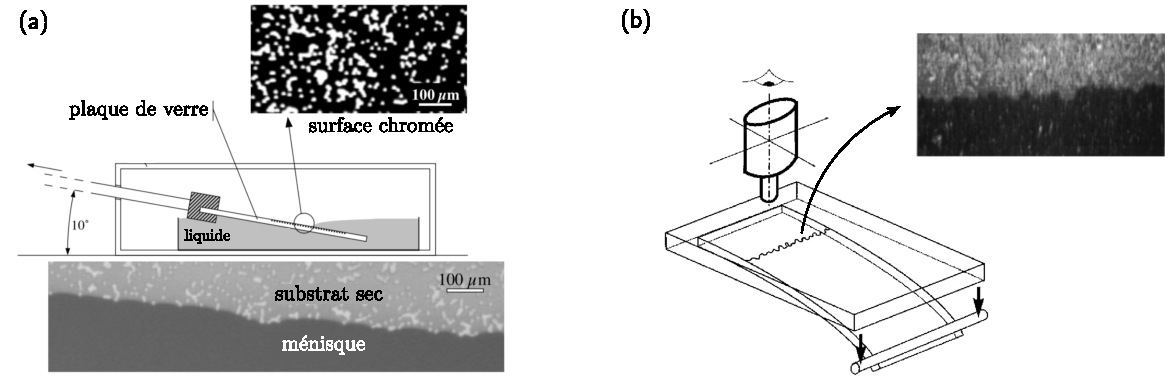
\includegraphics[width=\textwidth]{Chapitre1/Figures/Depinning/expdepinning.pdf}
	\caption{Illustrations des dispositifs expérimentaux permettant l'observation de la transition de depinning dans des conditions réelles. (a) Expérience (et figure) tirée de \cite{moulinet_roughness_2002} sur la propagation d'une ligne de mouillage. (b) Expérience (et figure) tirée de \cite{schmittbuhl_direct_1997} sur la propagation d'un front de fracture solide dans un bloc de plexiglas.}
	\label{fig:expdepinning}
\end{figure}

\paragraph{Propagation d'une fracture}

\subparagraph{}La propagation des fractures dans les solides désordonnés représente un autre exemple de la transition de dépiégeage. Dans l'exemple présenté à la \autoref{fig:expdepinning}-(b), un matériau est fracturé selon un mode I de fracture \cite{le_priol_long_range_2020}, i.e. en tirant une plaque perpendiculairement à la direction de propagation du front de fracture. Dans ce cadre, la limite entre les deux morceaux du solide peut être associée à une interface soumise au phénomène de dépiégeage. On y retrouve en effet tous les ingrédients nécessaires à cette transition : une force de rappel élastique exercée via l'élasticité du solide en volume, une force extérieure via la traction de la plaque inférieure, et une force de piégeage aléatoire directement associée à la structure amorphe du solide.

\subparagraph{}Comme pour le phénomène de mouillage, des expériences réelles ont permis d'étudier la propagation de ce front \cite{schmittbuhl_direct_1997, delaplace_high_1999, santucci_fracture_2010, le_priol_universal_2020}. Dans ce cas, l'analyse de la dynamique de l'interface et de sa rugosité a permis de confirmer sa compréhension dans le cadre de la théorie de la transition de dépiégeage.

\section{Propagateur de Eshelby}

\label{sec:Annexe_Eshelby}

\subparagraph{}Dans cette sous-section, nous présentons en détail le calcul du propagateur d'Eshelby dont la forme a été introduite à la \autoref{sec:ref_interac_elast}.

\subparagraph{}Afin de comprendre comment la contrainte est redistribuée dans le milieu au cours d'un réarrangement plastique dans le cadre de la transition vers l'écoulement, nous présentons la résolution de ce problème, déjà abordée à de nombreuses reprises dans la littérature, dans le cadre de la théorie de l'élasticité linéaire. Le problème initial est alors le suivant : comment est modifié le champ de contrainte local $\sigma$ sous forçage suite à une déformation plastique locale $\epsilon^\text{pl}$ ?

\subparagraph{}Pour répondre à cette question, nous reprenons les calculs des travaux \cite{picard_elastic_2004, goff_flow_2021}. Considérons un milieu continu élastique infini, isotrope et incompressible dans lequel nous définissons un champ de déplacement $u_i(\mathbf{r}) = u_i^\text{él}(\mathbf{r}) + u_i^\text{pl}(\mathbf{r})$, décomposable en une composante élastique et une composante plastique. \`A ce champ est associé un tenseur de déformation $\epsilon_{ij}$ défini comme :

\begin{equation}
	\epsilon_{ij}(\mathbf{r}) = \epsilon^\text{él}_{ij}(\mathbf{r})+\epsilon^\text{pl}_{ij}(\mathbf{r}) = \frac{1}{2}\left( \partial_i u_j^\text{él}(\mathbf{r}) + \partial_j u_i^\text{él}(\mathbf{r}) \right) + \frac{1}{2}\left( \partial_i u_j^\text{pl}(\mathbf{r}) + \partial_j u_i^\text{pl}(\mathbf{r}) \right)
	\label{eq:tenseurdeformation}
\end{equation}

et un tenseur des contraintes $\sigma_{ij}$ défini via la condition d'incompressibilité comme :

\begin{equation}
	\sigma_{ij}(\mathbf{r}) = 2\mu\epsilon^\text{él}_{ij}(\mathbf{r}) = 2\mu\epsilon_{ij}(\mathbf{r}) - 2\mu \epsilon^\text{pl}_{ij}(\mathbf{r})
	\label{eq:tenseurcontrainte}
\end{equation}

\subparagraph{}Dans le cas de notre étude, il est d'usage de décomposer les champs dans le milieu en une partie de réponse purement élastique au forçage extérieur ($\sigma^0$, $u^0$) et une partie de réponse à la déformation plastique ($\sigma^1$, $u^1$), donnant alors avec ces notations :

\begin{equation}
	\epsilon_{ij}^{\text{él}} = \epsilon_{ij}^{\text{él}, 0} + \epsilon_{ij}^{\text{él}, 1}, \quad \epsilon_{ij}^{\text{pl}} = \epsilon_{ij}^{\text{pl}, 1}, \quad \sigma_{ij} = \sigma_{ij}^0 + \sigma_{ij}^1
\end{equation}

\noindent L'effet non-trivial de la déformation plastique est alors encodé dans les équations :

\begin{equation}
\left\{
\begin{aligned}
	-\partial_i P^1(\mathbf{r}) + \partial_j\sigma_{ij}^1(\mathbf{r}) &= 0\\
	\partial_k u^1_k(\mathbf{r})&=0
	\end{aligned}
	\right.
\end{equation}

\noindent la première équation correspondant à la condition d'équilibre mécanique et la seconde à l'incompressibilité du matériau. L'objectif est alors de déterminer $\sigma_{ij}^1$ en fonction de $\epsilon_{ij}^{\text{pl},1}$ à partir de ces équations. Dans la suite, nous omettrons les notations $^1$ et $(\mathbf{r})$ pour alléger l'écriture.

\subparagraph{}En utilisant l'\autoref{eq:tenseurdeformation} et l'\autoref{eq:tenseurcontrainte}, nous pouvons ré-exprimer la condition d'équilibre mécanique comme suit :

\begin{equation}
	-\partial_i P + \mu \partial_j\partial_j u_i = 2\mu \partial_j\epsilon_{ij}^\text{pl}
\end{equation}

\noindent En passant dans l'espace de Fourier, avec les conventions exposées dans la \autoref{sec:conv_fourier}, on obtient grâce à la condition d'incompressibilité :

\begin{equation}
	\hat{P} = -2\mu\frac{q_iq_j}{q^2}\hat{\epsilon}_{ij}^\text{pl}
\end{equation}

\noindent soit :

\begin{equation}
	\hat{u}_i = \left( q_j\hat{\epsilon}_{ij}^\text{pl}-q_i\frac{q_\alpha q_\beta}{q^2}\hat{\epsilon}_{\alpha\beta}^\text{pl} \right)\frac{2i}{q^2}
\end{equation}

\noindent En se rapportant à la définition du tenseur des contraintes dans l'espace de Fourier on a alors finalement :

\begin{equation}
\begin{aligned}
	\hat{\sigma}_{ij} &= 2\mu \hat{G}_{ijkl}\hat{\epsilon}_{kl}^\text{pl}\\
	\hat{G}_{ijkl} &= \frac{q_i q_l\delta_{kj}+q_j q_l\delta_{ki}}{q^2}-2\frac{q_iq_jq_kq_l}{q^4}-\delta_{ki}\delta{jl}
\end{aligned}
\label{eq:eshelbygene}
\end{equation}

\subparagraph{}Afin d'obtenir une expression finale du champ de contrainte suite au réarrangement plastique, nous faisons l'hypothèse que celui-ci possède la même symétrie que le forçage, que nous prenons comme un cisaillement simple dans la direction $\hat{\mathbf{e}}_x$. Sous cette hypothèse, on a alors en deux dimensions $\hat{\epsilon}_{xy}^\text{pl} = \hat{\epsilon}_{yx}^\text{pl} = \hat{\epsilon}^\text{pl} \neq 0$ et $\hat{\epsilon}_{xx}^\text{pl} = \hat{\epsilon}_{yy}^\text{pl} = 0$. L'\autoref{eq:eshelbygene} nous permet alors d'obtenir l'expression :

\begin{equation}
	\hat{\sigma}_{xy} = 2\mu \hat{G} \epsilon^\text{pl}, \quad \hat{G}(\mathbf{q}) = -4\frac{q_x^2q_y^2}{q^4}
\end{equation}

\noindent qui relie directement la perturbation du champ de contrainte au réarrangement plastique. Des expressions similaires peuvent être obtenues pour les composantes $\sigma_{xx}$ et $\sigma_{yy}$ du tenseur des contraintes. En espace réel, cette relation devient :

\begin{equation}
	\sigma_{xy}(\mathbf{r}) = \int\mathrm{d}\mathbf{r}^\prime~G(\mathbf{r}-\mathbf{r}^\prime)\epsilon^\text{pl}(\mathbf{r}^\prime), \quad G(\mathbf{r}) = \frac{\cos (4\theta)}{\pi r^2}
	\label{eq:EshelbyReel}
\end{equation}

\subparagraph{}On appelle alors le propagateur $G$ propagateur d'Eshelby. Celui-ci correspond à la redistribution de contrainte de cisaillement induite par un réarrangement plastique infiniment localisé (de la forme $\epsilon^\text{pl}(\mathbf{r}) = \epsilon_0 \delta (\mathbf{r})$) ou de manière équivalente à celle induite en champ lointain par un évènement d'extension finie.

\section{Propagateurs hydrodynamiques}

\label{sec:Annexe_Interactions_Hydro}

\subparagraph{}Dans cette partie, nous développons le raisonnement dont les conclusions ont été exposées à la \autoref{sec:ref_interac_visc}. Nous proposons donc de montrer que l'interaction hydrodynamique entre deux particule immergées dans un fluide est génériquement à longue portée. En commençant par dériver sa forme dans le cas idéal, nous montrerons comment un raisonnement basé sur des principes simples de conservation permet d'appliquer cette analyse à toute une zoologie de systèmes, confirmant l'omniprésence de la longue portée dans les dispositifs expérimentaux et donc, a fortiori, dans la transition de réversibilité.

\paragraph{Hydrodynamique en milieu infini}

\subparagraph{}Dans le cas de la transition de réversibilité, lorsqu'une particule interagit irréversiblement avec une autre particule au cours d'un cycle, elle quitte son orbite initiale en appliquant une certaine force sur le fluide. Cette force va alors modifier l'écoulement du fluide via les lois régissant sa dynamique et donc affecter le mouvement des particules environnantes. La question est de savoir comment. Pour y répondre, nous nous concentrons sur un problème générique à deux particules : une particule $1$ située en $\mathbf{r}$ exerce une force $\mathbf{F}^1(\mathbf{r})$ sur le fluide et induit un écoulement qui entraîne le déplacement d'une particule $2$ située en $\mathbf{r}^\prime$ à la vitesse $\mathbf{v}^2$. En considérant le fluide suspendant comme incompressible et dans la limite de bas Reynolds, son écoulement suit une dynamique régie par les équations de Stokes :

\begin{equation}
\begin{aligned}
	-\partial_i P + \eta \partial_j\partial_j v_i + f_i &= 0 \\
	\partial_j v_j = 0
\end{aligned}
\end{equation}

\noindent avec $\mathbf{v}(\mathbf{r})$ le champ de vitesse eulérien du fluide, $P(\mathbf{r})$ le champ de pression, $\eta$ la viscosité dynamique et $\mathbf{f}(\mathbf{r})$ le champ de force extérieur. Dans la limite de champ lointain, i.e. à grande distance des particules, celles-ci peuvent être assimilées à des objets ponctuels. Dans cette approximation, nous pouvons décrire la force exercée par la particule $1$ sur le fluide comme infiniment localisée $\mathbf{F}^1(\mathbf{r}) = \mathbf{F}^1\delta (\mathbf{r})$ et la vitesse de la particule $2$ comme correspondant à celle du fluide en ce point $\mathbf{v}^2 = \mathbf{v}(\mathbf{r}^\prime)$ \cite{diamant_hydrodynamic_2009}. La résolution de ce problème revient donc à résoudre les équations de Stokes pour obtenir le champ de vitesse du fluide en $\mathbf{r}^\prime$ sous l'action du champ de force extérieur $\mathbf{f}(\mathbf{r}) = \mathbf{F}^1\delta (\mathbf{r})$. En d'autres termes, cela revient à calculer la fonction de Green associée aux équations de Stokes \cite{noauthor_physique_nodate}.

\subparagraph{}La résolution de ce problème bien connu (voir \cite{lisicki_four_2013} par exemple) permet de définir le tenseur d'Oseen $G_{ij}$, reliant $\mathbf{F}^1$ à $\mathbf{v}(\mathbf{r}^\prime)$ par la relation linéaire :

\begin{equation}
	v_i (\mathbf{r}^\prime) = G_{ij}(\mathbf{r} -\mathbf{r}^\prime)F^1_j, \quad G_{ij}(\mathbf{r}) = \frac{1}{8\pi\eta r}\left( \delta_{ij}+\frac{r_ir_j}{r^2} \right)
\end{equation}

\noindent définissant ainsi une interaction hydrodynamique entre les deux particules, décroissant comme $\sim 1/r$ dans un milieu tridimensionnel infini.

\subparagraph{}Ce résultat calculatoire peut aussi se comprendre plus intuitivement, comme l'explique très clairement l'étude \cite{diamant_hydrodynamic_2009}. Dans la suite de cette partie, nous présentons le raisonnement de l'auteur. En fait, les équations de Stokes dérivent de deux lois de conservation fondamentales : celle de la quantité de mouvement et celle de la masse. Lorsqu'une particule applique une force locale sur le fluide, celle-ci se comporte comme une source de quantité de mouvement. Pour que cette dernière soit conservée, le flux local de quantité de mouvement émanant de la particule doit décroître comme $\sim 1/r^2$ en 3D. Or ce flux local de quantité de mouvement n'étant autre que le tenseur des contraintes $\sigma$ associé au fluide, cette conservation implique directement $\sigma \sim 1/r^2$. La partie associée au cisaillement de ce tenseur étant $\sigma_\text{cis}\sim \eta \mathbf{\nabla} \mathbf{v}$ on a donc $\mathbf{v}\sim 1/\eta r$. De plus, par des considérations de symétrie, la partie adimensionnelle du propagateur hydrodynamique prend nécessairement la forme $\delta_{ij}+C\frac{r_ir_j}{r^2}$. On retrouve donc finalement, basé sur ces arguments simples :

\begin{equation}
	G_{ij} \sim \frac{1}{\eta r}\left( \delta_{ij}+C\frac{r_ir_j}{r^2} \right)
	\label{eq:diamantinfini}
\end{equation}

\noindent avec $C$ une constante qui peut être déterminée par conservation de la masse (en imposant $\partial_i G_{ij}=0$) pour donner $C=1$.

\subparagraph{}En plus de ce premier effet, nous pouvons identifier une autre source de modification de l'écoulement. Celle-ci vient de la conservation de la masse de fluide. En fait, lors de son déplacement, la particule $1$ modifie la répartition de masse dans le fluide. Celle-ci peut alors être vue, en plus d'une source de quantité de mouvement, comme un dipôle de source de matière (avec création de masse à l'avant du mouvement et suppression de masse à l'arrière). En 3D, un tel dipôle génère une vitesse d'écoulement décroissant comme $\sim 1/r^3$, générant ainsi un terme additionnel à l'\autoref{eq:diamantinfini} en $\sim 1/r^3$. Cependant, à grande distance, cette contribution est négligeable devant celle décroissant comme $\sim 1/r$. On retrouve donc bien en champ lointain le tenseur d'Oseen.

\subparagraph{}Ce résultat basé sur les deux principes de conservation sont très généraux et permettent facilement d'étendre leur validité à d'autre situations. Notamment, dans une suspension de plus de deux particules, la forme de l'interaction en champ lointain ne sera pas modifiée puisque dans ce cas on a toujours conservation de la quantité de mouvement et de la masse \cite{diamant_hydrodynamic_2009}. A priori, dans un système assimilé à un milieu infini, les interactions hydrodynamiques entre les particules lors d'un cycle de cisaillement sont donc bien à longue portée. Toutefois une telle approximation de milieu infini est parfois non valable dans les dispositifs expérimentaux réalisant la transition de réversibilité. Dans ces cas là, le raisonnement doit être adapté.

\paragraph{Hydrodynamique en milieux complexes}

\subparagraph{}Un premier exemple vient des systèmes quasi-2D. Lorsque le fluide suspendant est confiné entre deux plaques rigides, espacées d'une faible distance $\lambda$, les frottements avec le solide constituent une perte de quantité de mouvement dans la direction orthogonale aux plaques. Dans ce cas, le flux local de quantité de mouvement généré par la particule $1$ décroît exponentiellement avec la distance au-delà de cette distance typique de confinement $r>\lambda$. Toutefois, dans une telle configuration, la masse du fluide est toujours conservée. Le déplacement de la particule $1$ peut toujours être vu comme un dipôle de source de matière mais prenant cette fois place dans un milieu 2D. La vitesse de l'écoulement associé décroît alors comme $\sim 1/r^2$, amenant à un propagateur hydrodynamique de la forme :

\begin{equation}
	G_{ij} \sim \frac{1}{\eta r^2}\left( \delta_{ij}-2\frac{r_ir_j}{r^2} \right)
\end{equation}

\noindent Ainsi, sous confinement, les interactions médiées par le fluide restent à longue portée.

\subparagraph{}Un autre système envisageable est celui d'un fluide contenu dans un film suspendu (i.e. entouré de gaz par exemple, comme dans une bulle de savon). Dans ce cas, la quantité de mouvement et la masse sont conservées mais l'écoulement prend place dans un milieu 2D. La conservation de la quantité de mouvement implique donc cette fois un flux local évoluant comme $\sim 1/r$ et donc une vitesse d'écoulement se comportant comme $\sim \ln (r)$, soit des interactions d'une portée extrêmement grande.

\subparagraph{}Enfin une dernière situation envisageable, bien que peut-être moins pertinente dans le cas de la transition de réversibilité, est celle d'un écoulement dans un milieu poreux. Dans ce cas, la quantité de mouvement n'est pas conservée, comme dans le cas du confinement entre deux plaques, mais cette fois la conservation de la masse prend place dans un espace 3D. Dans ce cas, le raisonnement de conservation nous amène à un propagateur hydrodynamique décroissant comme $\sim 1/r^3$.

\subparagraph{}De manière toute à fait générale, le fluide suspendant permet donc de médier des interactions entre les particules, représentée par un propagateur hydrodynamique de la forme :

\begin{equation}
	G_{ij} \sim \frac{1}{r^\gamma}\left( \delta_{ij}-2\frac{r_ir_j}{r^2} \right)
\end{equation}

\noindent avec $\gamma$ un entier pouvant prendre différentes valeurs en fonction du dispositif spécifique étudié. Via a minima la conservation de la masse, ces interactions présentent donc toujours la particularité d'être à longue portée. 

\subparagraph{}Dans une modélisation plus spécifique de la transition de réversibilité, les interactions irréversibles de contact entre deux particules peuvent être vues comme des dipôles de force sur le fluide. Les résultats présentés précédemment sont alors modifiés selon $\gamma \rightarrow \gamma +1$. Par exemple, en milieu 3D infini, nous nous attendons à ce qu'un évènement affecte les autres particules du système via une interaction décroissant comme $\sim 1/r^2$.

\FloatBarrier

\chapter{Annexes au chapitre 2}

\section{Mesures d'hyperuniformité dans le modèle LR-Manna}

\label{sec:mesures_HU_Manna}

\subparagraph{}Dans cette section, nous présentons les résultats obtenus dans le cadre de l'étude de l'hyperuniformité dans les modèles LR-Manna. Plus précisément, nous présentons sur les figures suivantes les redimensionnements obtenus de la même façon que dans le cas $\alpha=4$ représenté par la \autoref{fig:MannaCMHU_rescale_gamma4} mais pour d'autres valeurs de la portée du transport.

\begin{figure}[H]
	\centering
	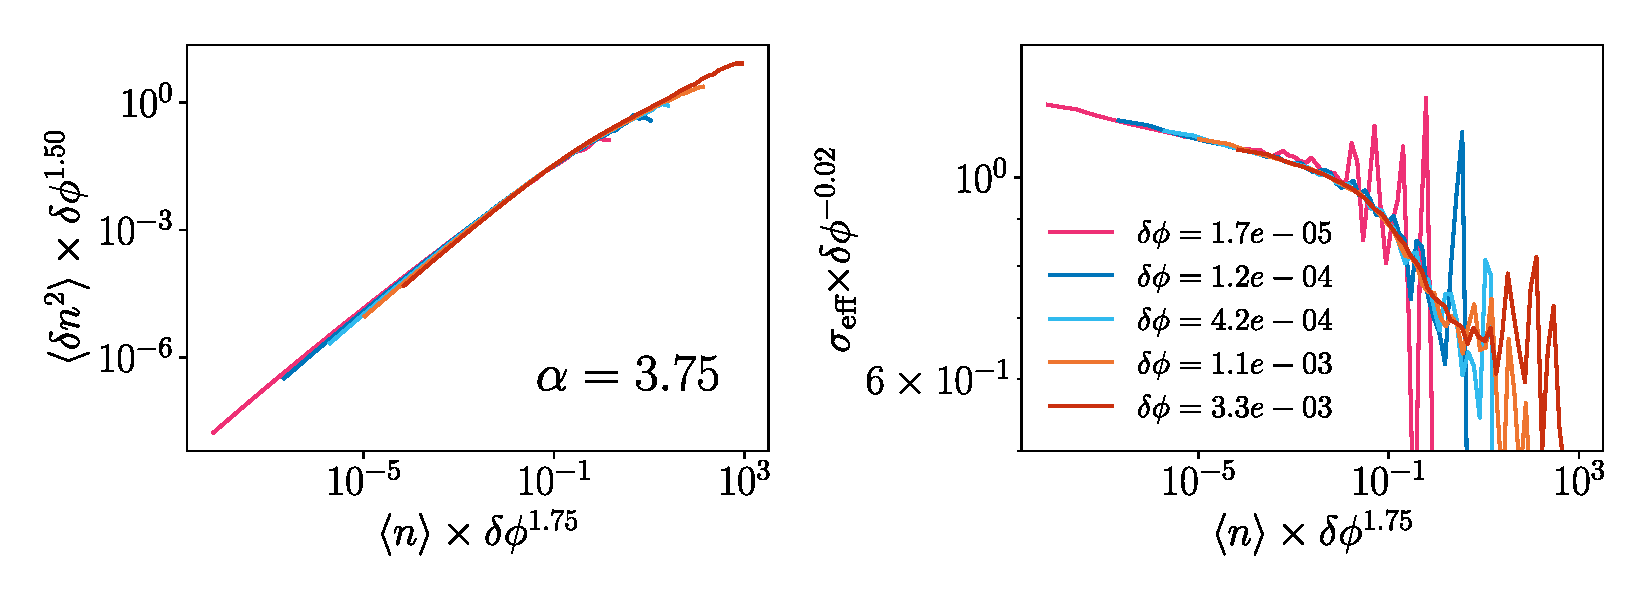
\includegraphics[width=\textwidth]{Chapitre2/Figures/Hyperuniformity/RescaleHU_MannaCM_Gamma375.pdf}
	\caption{Idem que la \autoref{fig:MannaCMHU_rescale_gamma4}, seulement pour $\alpha=3.75$}
	\label{fig:MannaCMHU_rescale_gamma375}
\end{figure}

\begin{figure}[H]
	\centering
	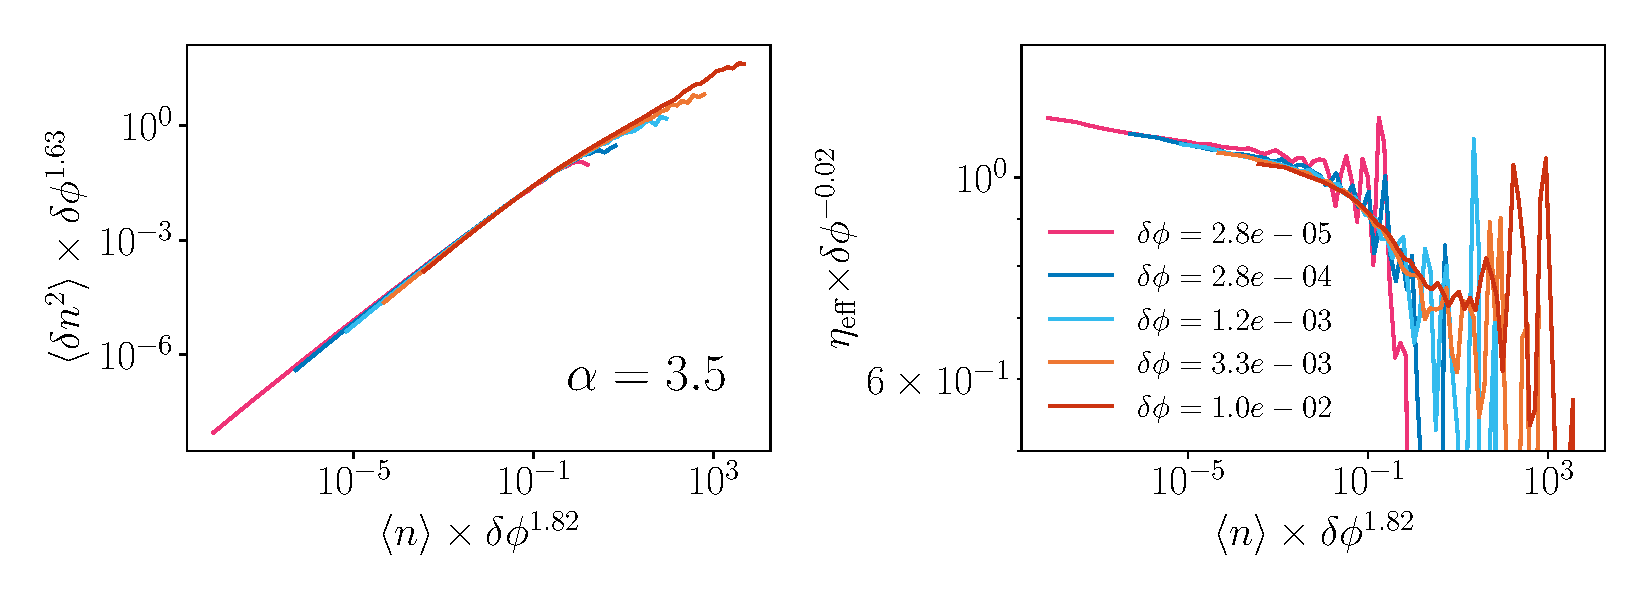
\includegraphics[width=\textwidth]{Chapitre2/Figures/Hyperuniformity/RescaleHU_MannaCM_Gamma35.pdf}
	\caption{Idem que la \autoref{fig:MannaCMHU_rescale_gamma4}, seulement pour $\alpha=3.5$}
	\label{fig:MannaCMHU_rescale_gamma35}
\end{figure}

\begin{figure}[H]
	\centering
	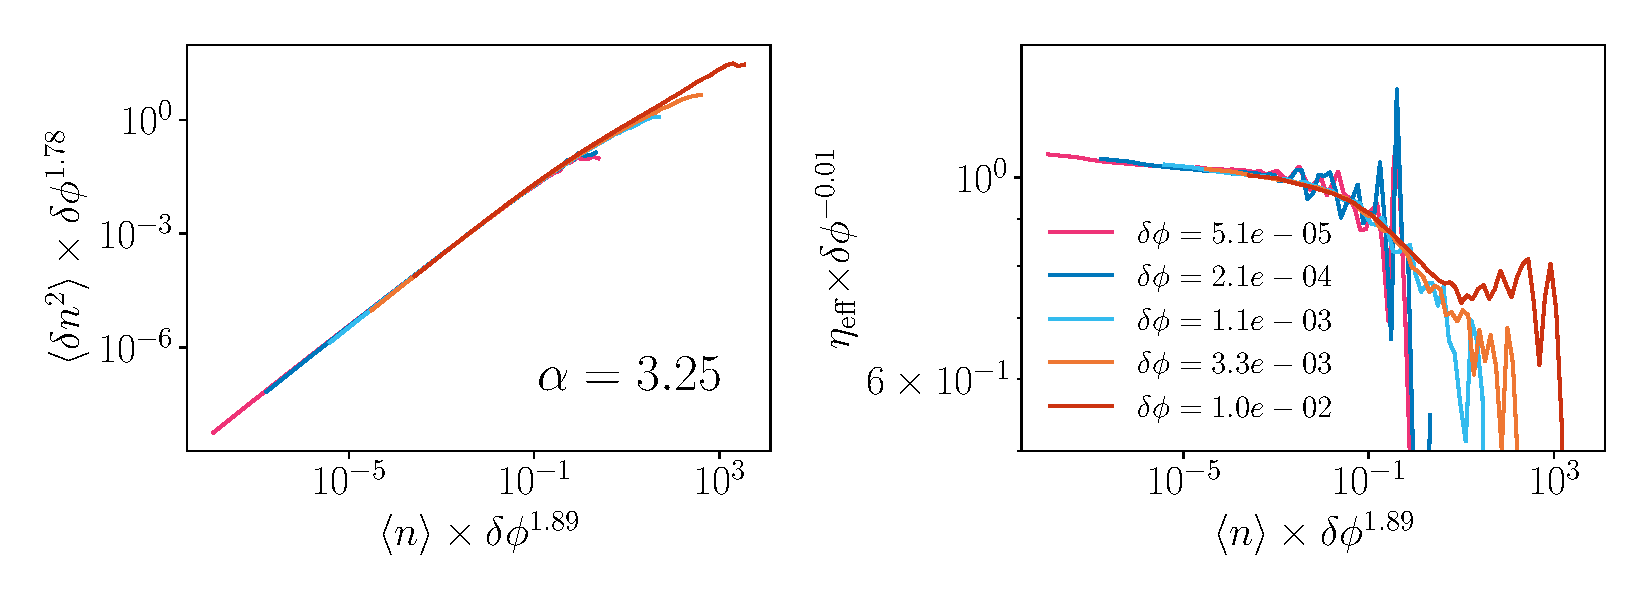
\includegraphics[width=\textwidth]{Chapitre2/Figures/Hyperuniformity/RescaleHU_MannaCM_Gamma325.pdf}
	\caption{Idem que la \autoref{fig:MannaCMHU_rescale_gamma4}, seulement pour $\alpha=3.25$}
	\label{fig:MannaCMHU_rescale_gamma325}
\end{figure}

\begin{figure}[H]
	\centering
	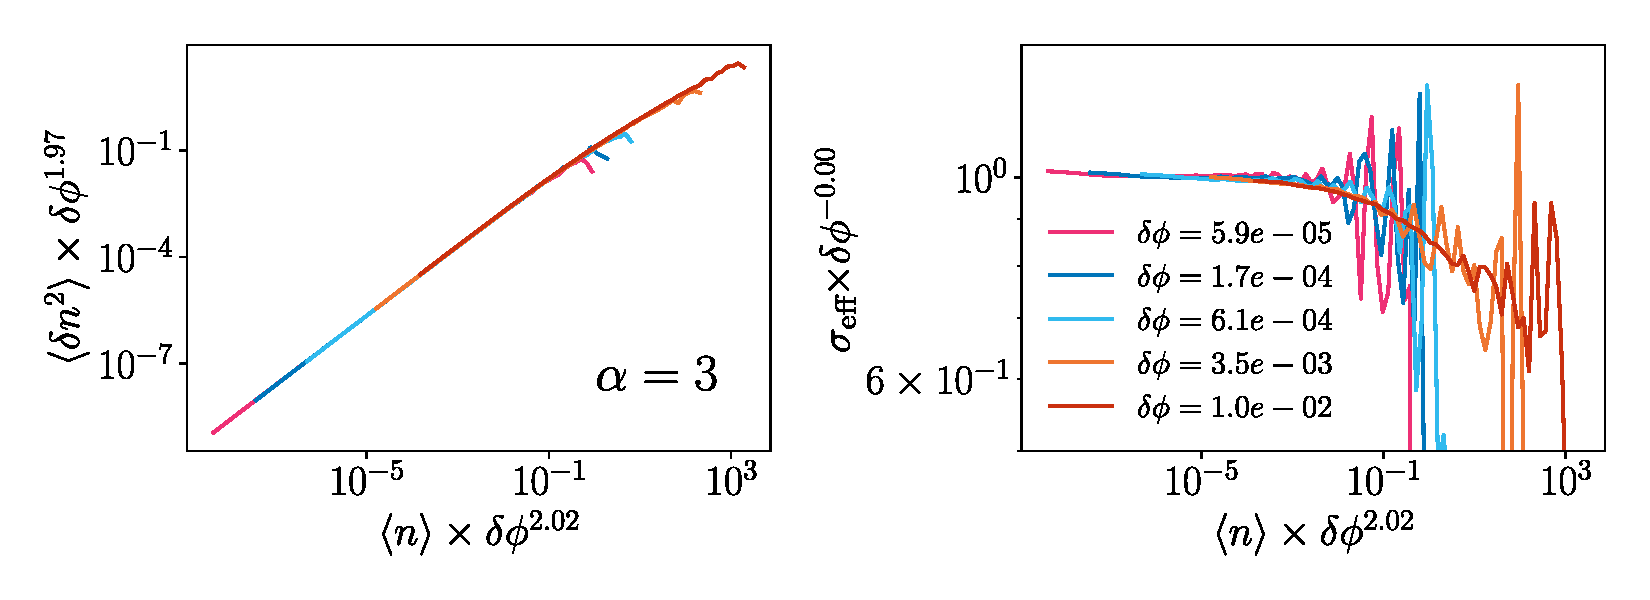
\includegraphics[width=\textwidth]{Chapitre2/Figures/Hyperuniformity/RescaleHU_MannaCM_Gamma3.pdf}
	\caption{Idem que la \autoref{fig:MannaCMHU_rescale_gamma4}, seulement pour $\alpha=3$}
	\label{fig:MannaCMHU_rescale_gamma3}
\end{figure}

\FloatBarrier

\chapter{Annexes au chapitre 3}

\section{Transformée de Fourier des propagateurs}

\label{sec:TFinverse_susp}

\subparagraph{}Dans cette sous-section, nous présentons le calcul dans l'espace continu de la transformée de Fourier des propagateurs $\mathcal{G}^2$ utilisés dans le $\alpha$-ROM et donnés par :

\begin{equation}
	\mathcal{G}^2(\mathbf{r}) = \frac{c}{\left(1+\left(\frac{r}{D_p}\right)^2\right)^\alpha}, \quad c > 0
\end{equation}

\noindent Nous prenons alors $D_p = 1$ (comme dans nos simulations numériques) et notons $f(\mathbf{r}) = \mathcal{G}^2(\mathbf{r})$ pour alléger l'écriture.

\subparagraph{}Nous commençons par utiliser le lien entre transformée de Fourier d'une fonction radiale et transformée de Hankel \cite{poularikas_transforms_2018} permettant d'obtenir\footnote{Il suffit, à partir de la définition de la transformée de Fourier, de faire l'intégrale sur la variable angulaire $\theta$ qui permet d'obtenir la fonction de Bessel de première espèce.} :

\begin{equation}
	\hat{f}(\mathbf{q}) = q^{\frac{2-D}{2}}(2\pi)^{\frac{D}{2}}\int\mathrm{d}r~J_{\frac{D-2}{2}}(qr)r^\frac{D-2}{2}f(\mathbf{r})r
\end{equation}

\noindent qui dans notre cas amène à : 

\begin{equation}
	\hat{f}(\mathbf{q}) = c q^{\frac{2-D}{2}}(2\pi)^{\frac{D}{2}}\int\mathrm{d}r~J_{\frac{D-2}{2}}(qr)\frac{r^\frac{D}{2}}{(1+r^2)^\alpha}
\end{equation}

\noindent Puis nous utilisons le résultat suivant concernant les fonctions de Bessel \cite{zwillinger_6_7_2014} :

\begin{equation}
\int_0^{\infty} \frac{J_\nu(b x) x^{\nu+1}}{\left(x^2+a^2\right)^{\mu+1}} d x=\frac{a^{\nu-\mu} b^\mu}{2^\mu \Gamma(\mu+1)} K_{\nu-\mu}(a b), \quad -1 < \nu < 2\mu + \frac{3}{2}
\end{equation}

\noindent Par identification des deux équations on arrive alors directement à :

\begin{equation}
	\hat{f}(\mathbf{q}) = c q^{\frac{2-D}{2}}(2\pi)^{\frac{D}{2}}\frac{q^{\alpha-1}}{2^{\alpha - 1}\Gamma(\alpha)}K_{\frac{D-2}{2}-(\alpha-1)}(q)
\end{equation}

\noindent soit en simplifiant et en utilisant $K_\nu (q) = K_{-\nu}(q)$ :

\begin{equation}
	\hat{f}(\mathbf{q}) = \frac{(2\pi)^{\frac{D}{2}}}{2^{\alpha-1}\Gamma(\alpha)}q^{\alpha-\frac{D}{2}}K_{\alpha-\frac{D}{2}}(q), \quad \alpha > \frac{D-1}{4}
\end{equation}

\noindent ce qui nous permet bien de retrouver les expressions données au \autoref{chapter:Susp} pour $D=2$ et $D=3$.

\section{Résolution numérique du modèle $\mu$-Hébraud-Lequeux}

\label{sec:ResolNumMuHL}

\subparagraph{}Afin d'étudier le comportement critique du modèle $\mu$-Hébraud-Lequeux dans le cadre de la modélisation champ moyen du $\alpha$-ROM, nous proposons une méthode d'intégration numérique indirecte de l'\autoref{eq:muHL}. Dans le cas du modèle original de Hébraud-Lequeux, il est possible de résoudre les équations associées via une dynamique de population \cite{bouchaud_spontaneous_2016}. Dans cette partie, nous proposons de transposer cette méthode de résolution à l'intégration des équations du modèle $\mu$-Hébraud-Lequeux. En fait, l'équation suivante : 

\begin{equation}
\begin{aligned}
    \partial_t P(\mathbf{r}, t) &= -a\Gamma (t)|\nabla|^{\mu} P(\mathbf{r}, t) - \frac{1}{\tau}\Theta(|\mathbf{r}|>R)P(\mathbf{r}, t) + \delta(\mathbf{r})\Gamma (t)\\
     \Gamma (t) &= \frac{1}{\tau}\int_{|\mathbf{r}|>R}\mathrm{d}\mathbf{r}~P(\mathbf{r}, t)
\end{aligned}
\end{equation}

\noindent peut être vue comme une équation de Fokker-Planck. Suivant cette idée, nous pouvons associer à ce modèle une dynamique de Langevin simple sur la variable $\mathbf{r}$ qui permet, statistiquement, de reconstruire le comportement de la distribution $P$.

\subparagraph{}En pratique, nous considérons donc $N$ particules dont les positions $\mathbf{r}_i$ évoluent dans un espace de dimension $D$, présentant une barrière en $|\mathbf{r}|=R$. La dynamique du mouvement des particules se fait en temps continu, discrétisé selon un pas de temps $\Delta t$. \`A chaque pas de temps $t_i$, chaque particule effectue un saut distribué selon une loi de Lévy stable $S_\mu(0,c,0)$ définie par sa fonction caractéristique :

\begin{equation}
	\phi(k) = \exp (-|ck|^\mu)
\end{equation}

\noindent modélisant le terme en dérivée fractionnaire dans l'équation sur $P$ \cite{hinrichsen_non_equilibrium_2007, jespersen_levy_1999}. Par équivalence des deux descriptions, la constante $c$ est alors définie selon\footnote{\todo{expliquer la réflexion derrière vite fait}} :

\begin{equation}
	c = \left( s \Gamma(t) \Delta t \right)^{1/\mu}
\end{equation}

\noindent la constante $s$ dans la vision dynamique de population jouant un rôle similaire à la constante $a$ dans l'équation d'évolution de la distribution. Il est théoriquement possible de relier $a$ à $s$ mais ce n'est pas nécessaire dans notre cas puisque nous nous intéressons simplement au comportement critique associé. Lorsqu'une particule est au-delà de la barrière, celle-ci est remise à l'origine du repère selon un taux $1/\tau$, représentant alors les deux derniers termes du membre de droite dans l'équation de Fokker-Planck.

\subparagraph{}Dans ce modèle, les particules n'interagissent pas directement entre elles, mais indirectement via la distribution de sauts qui dépend de l'activité dans le système $\tau\Gamma (t)$. Celle-ci est calculée à chaque pas de temps comme la proportion de particules au-delà de la barrière située en $|\mathbf{r}|=R$. Nous représentons à la \autoref{fig:walker} La dynamique d'une de ces particules en 2D pour différentes valeurs de $\mu$.

\begin{figure}[h]
	\centering
	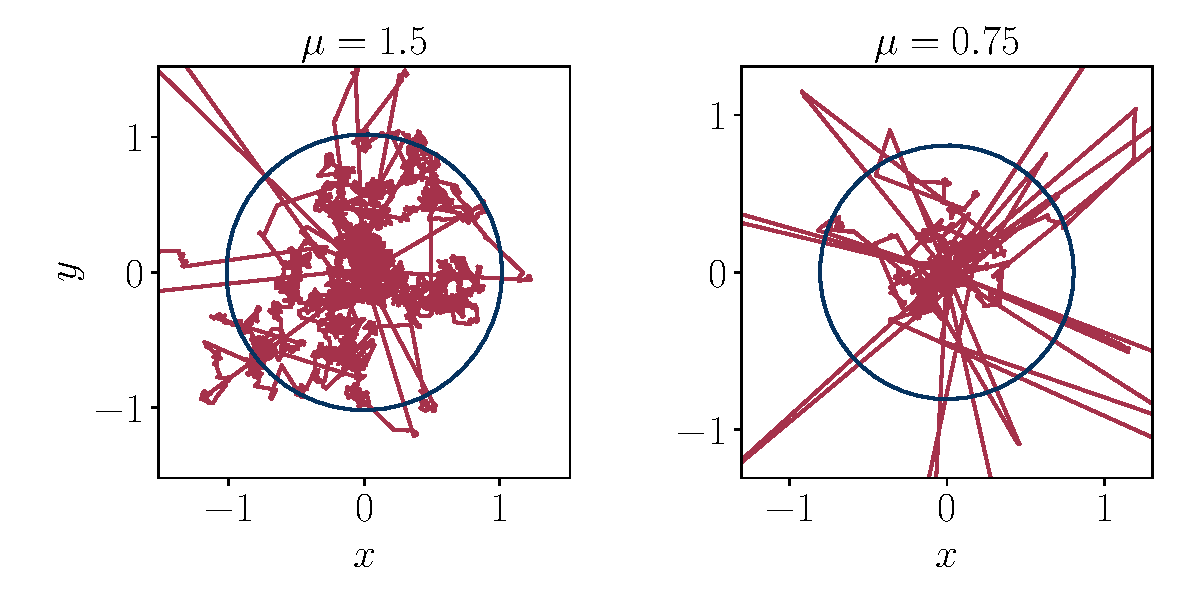
\includegraphics[width= 0.8\textwidth]{walker.pdf}
	\caption{Trajectoire d'une particule dans la résolution numérique des équations du modèle $\mu$-Hébraud-Lequeux via une dynamique de population pour $\mu = 1.5$ (panel de gauche) et $\mu = 0.75$ (panel de droite). Ces deux trajectoires correspondent à un état stationnaire de la dynamique de population avec une distance au point critique $\delta R = \frac{R_c-R}{R_c}\approx 10^{-1}$}
	 \label{fig:walker}
\end{figure}

\subparagraph{}En simulant le mouvement de ces particules, nous pouvons remonter à la forme instantanée de la distribution $P(\mathbf{r},t)$ prise alors comme la distribution des positions des différentes particules. Pour déterminer le comportement critique de cette transition, nous mesurons la valeur de l'activité moyenne $\Gamma$ dans l'état stationnaire pour différentes valeurs de $R$ afin d'identifier l'exposant $\beta$ définissant la relation :

\begin{equation}
	\Gamma \sim (R-R_c)^\beta
\end{equation}

\subparagraph{} Les résultats présentés à la \autoref{fig:LHLNum} ont été obtenus pour les valeurs des paramètres $s=1$, $\Delta t  = 10^{-2}$, $\tau = 1$ et $N \sim 10^7$. Dans le cas $\mu = 2$ où la loi stable devient une loi normale, nous vérifions que nous retrouvons les résultats attendus soit $\beta = 2$ et $R_c = \sqrt{2a}$, et la distribution stationnaire  prédite via la résolution analytique (rendue possible dans ce cas). Cela suggère la validité de notre approche.

\paragraph{Détails d'implémentation}

\subparagraph{}L'algorithme présenté a été implémenté en langage C++/CUDA pour fonctionner sur cartes graphiques. Les détails d'implémentation peuvent être retrouvés sur \textbf{lien github}. Les nombres aléatoires distribués selon des lois stables, utilisés pour générer les sauts des particules, ont été générés via la méthode Chambers-Mallows-Stuck \cite{chambers_method_1976, weron_chambers_mallows_stuck_1996}.

\section{Fonctions de corrélation de paire}

\label{sec:PCorr}

\subsection{$\alpha$-ROM en 2D avec sauts infinis des particules actives}

\subparagraph{}Dans cette partie, nous présentons les résultats obtenus concernant les mesures de fonctions de corrélation de paire entre particules passives dans le $\alpha$-ROM en 2D avec sauts infinis des particules actives. Sur les figures suivantes, nous présentons les meilleurs redimensionnements obtenus pour chaque portée $\alpha$, donnant lieu aux valeurs de l'exposant de pseudo-gap $\theta$ répertoriées sur la \autoref{fig:mueff}-(b).

\begin{figure}[h]
\centering
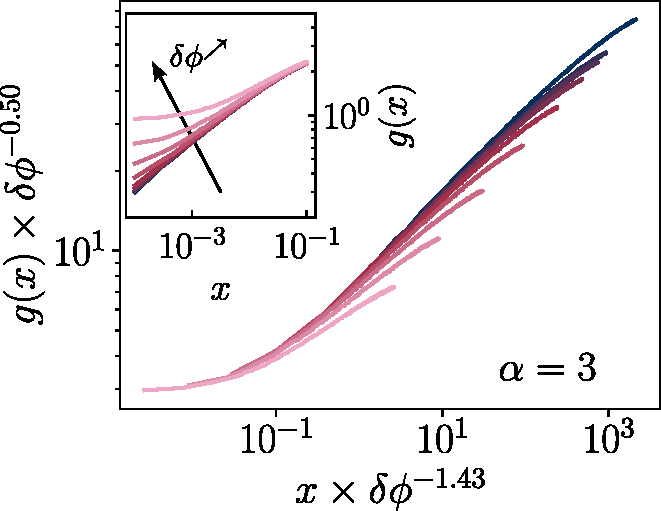
\includegraphics[width=0.45\textwidth]{Chapitre3/Figures/Interpretation/PCorrMF/PCorr_rescaled_MF_alpha3.pdf}
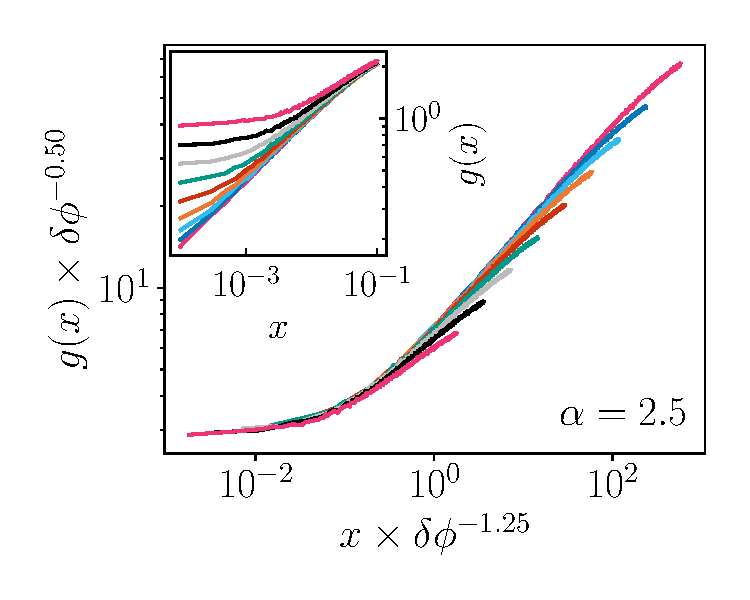
\includegraphics[width=0.45\textwidth]{Chapitre3/Figures/Interpretation/PCorrMF/PCorr_rescaled_MF_alpha25.pdf}
\caption{Idem que pour la \autoref{fig:PCorr_alphaMF} pour $\alpha = 3$ (gauche) et $\alpha = 2.5$ (droite)}
\label{fig:PCorrAnnexe1}
\end{figure}

\begin{figure}[h]
\centering
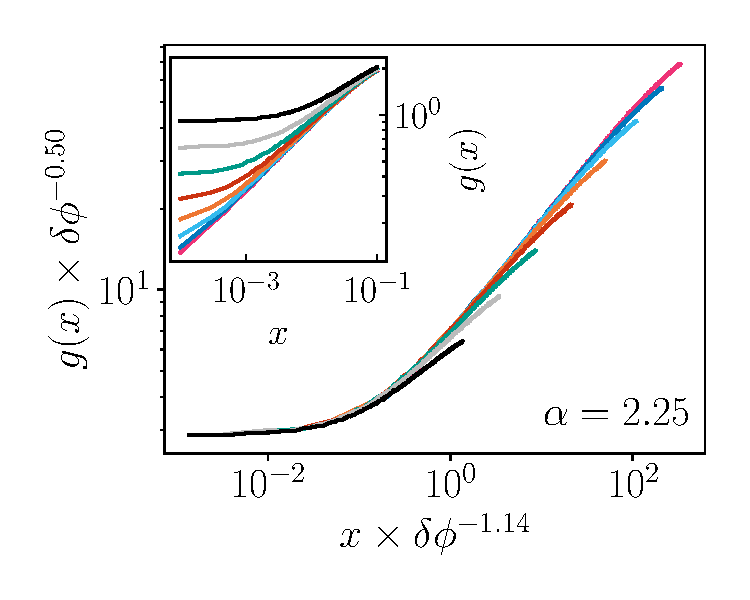
\includegraphics[width=0.45\textwidth]{Chapitre3/Figures/Interpretation/PCorrMF/PCorr_rescaled_MF_alpha225.pdf}
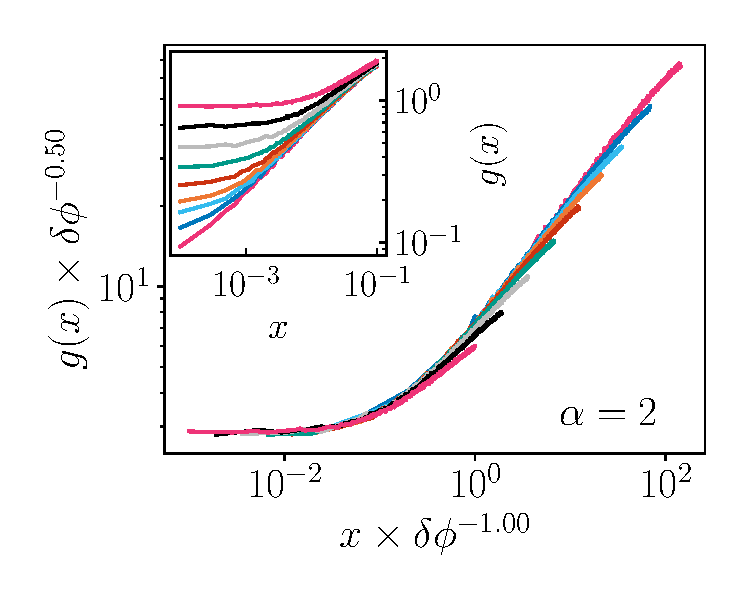
\includegraphics[width=0.45\textwidth]{Chapitre3/Figures/Interpretation/PCorrMF/PCorr_rescaled_MF_alpha2.pdf}
\caption{Idem que pour la \autoref{fig:PCorr_alphaMF} pour $\alpha = 2.25$ (gauche) et $\alpha = 2$ (droite)}
\label{fig:PCorrAnnexe2}
\end{figure}

\begin{figure}[h]
\centering
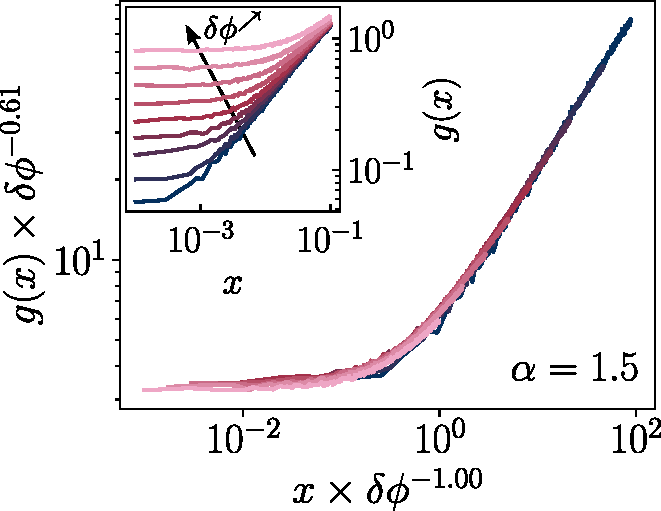
\includegraphics[width=0.45\textwidth]{Chapitre3/Figures/Interpretation/PCorrMF/PCorr_rescaled_MF_alpha15.pdf}
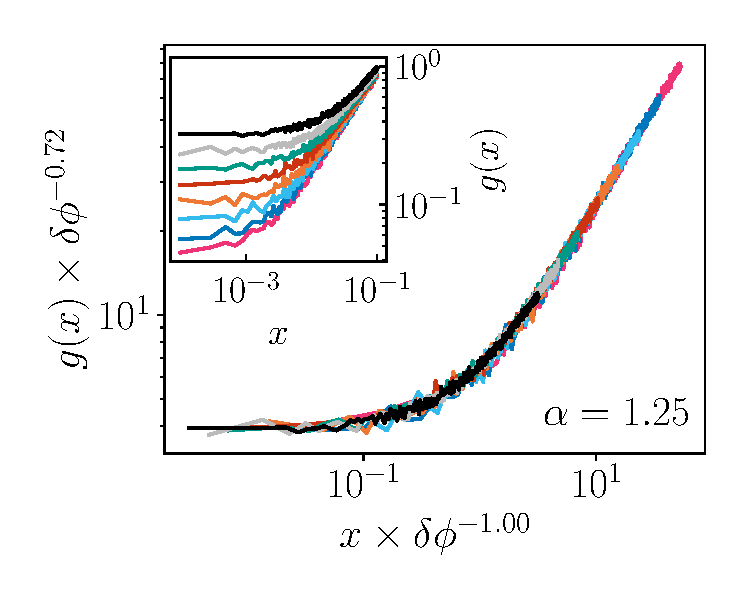
\includegraphics[width=0.45\textwidth]{Chapitre3/Figures/Interpretation/PCorrMF/PCorr_rescaled_MF_alpha125.pdf}
\caption{Idem que pour la \autoref{fig:PCorr_alphaMF} pour $\alpha = 1.5$ (gauche) et $\alpha = 1.25$ (droite)}
\label{fig:PCorrAnnexe3}
\end{figure}

\begin{figure}[h]
\centering
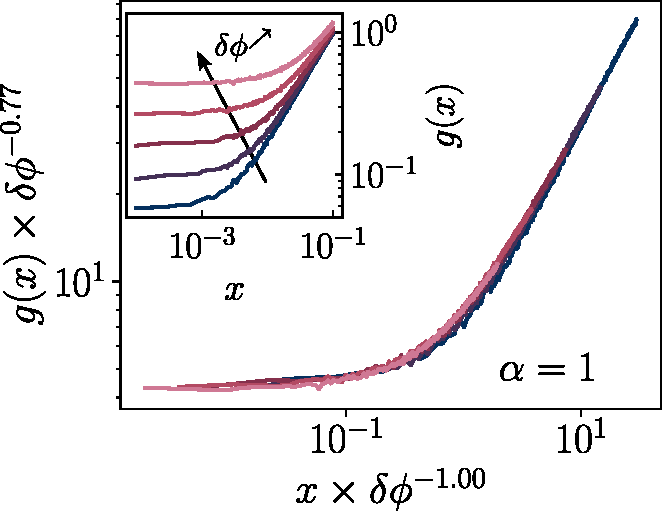
\includegraphics[width=0.45\textwidth]{Chapitre3/Figures/Interpretation/PCorrMF/PCorr_rescaled_MF_alpha1.pdf}
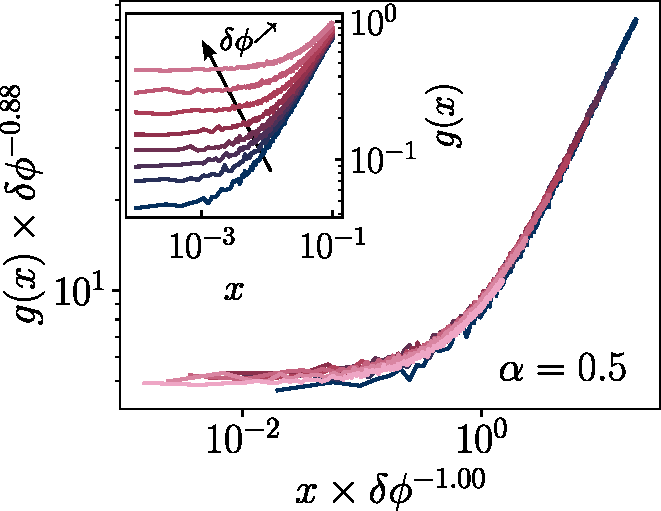
\includegraphics[width=0.45\textwidth]{Chapitre3/Figures/Interpretation/PCorrMF/PCorr_rescaled_MF_alpha05.pdf}
\caption{Idem que pour la \autoref{fig:PCorr_alphaMF} pour $\alpha = 1$ (gauche) et $\alpha = 0.5$ (droite)}
\label{fig:PCorrAnnexe4}
\end{figure}

\FloatBarrier

\subsection{$\alpha$-ROM en 2D avec sauts finis des particules actives}

\subparagraph{}Dans cette partie, nous présentons les résultats obtenus concernant les mesures de fonctions de corrélation de paire entre particules passives dans le $\alpha$-ROM en 2D avec sauts finis des particules actives. Sur les figures suivantes, nous présentons les meilleurs redimensionnements obtenus pour chaque portée $\alpha$, donnant lieu aux valeurs de l'exposant de pseudo-gap $\theta$ répertoriées sur la \autoref{fig:Beta_Theta}.

\begin{figure}[h]
\centering
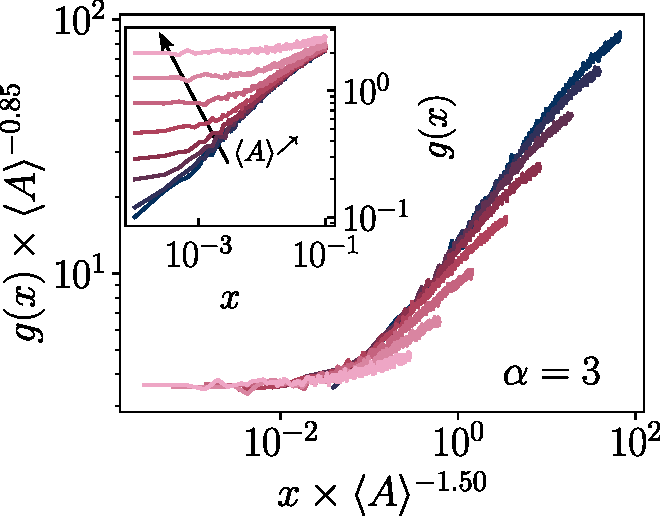
\includegraphics[width=0.45\textwidth]{Chapitre3/Figures/Interpretation/PCorr/PCorr_rescaled_alpha3_mean.pdf}
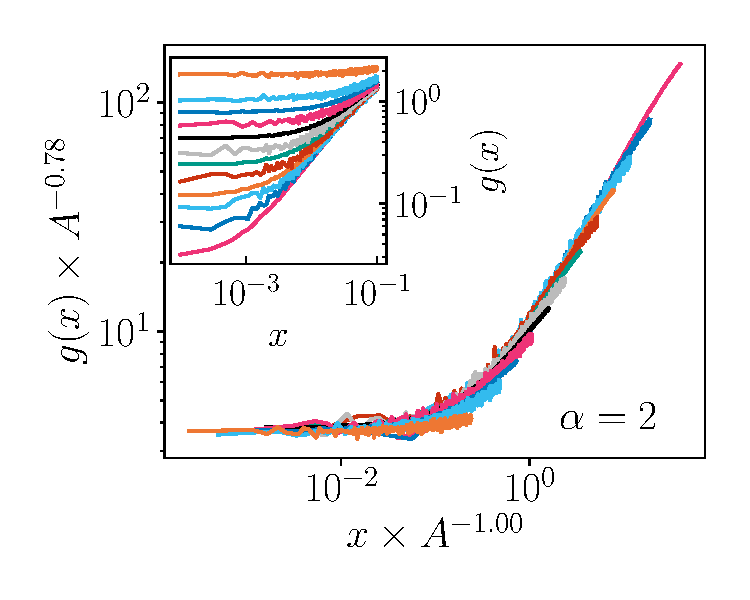
\includegraphics[width=0.45\textwidth]{Chapitre3/Figures/Interpretation/PCorr/PCorr_rescaled_alpha2_mean.pdf}
\caption{Idem que pour la \autoref{fig:PCorr_alpha} pour $\alpha = 3$ (gauche) et $\alpha = 2$ (droite)}
\label{fig:PCorrAnnexe5}
\end{figure}

\begin{figure}[h]
\centering
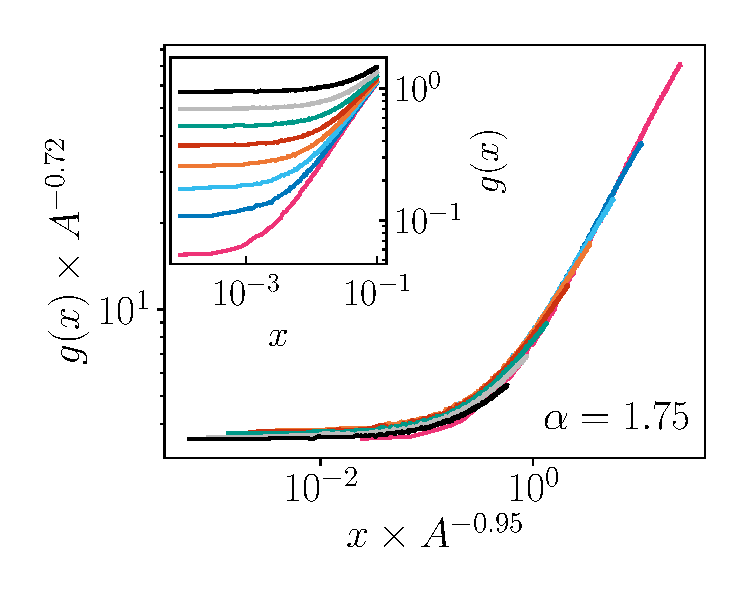
\includegraphics[width=0.45\textwidth]{Chapitre3/Figures/Interpretation/PCorr/PCorr_rescaled_alpha175_mean.pdf}
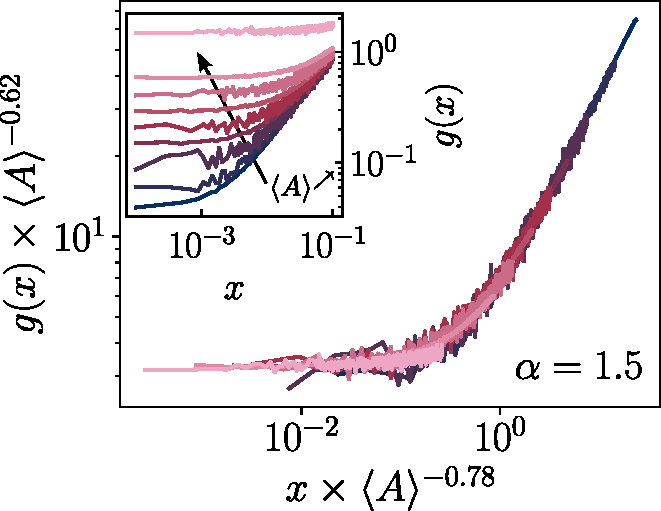
\includegraphics[width=0.45\textwidth]{Chapitre3/Figures/Interpretation/PCorr/PCorr_rescaled_alpha15_mean.pdf}
\caption{Idem que pour la \autoref{fig:PCorr_alpha} pour $\alpha = 1.75$ (gauche) et $\alpha = 1.5$ (droite)}
\label{fig:PCorrAnnexe5}
\end{figure}

\begin{figure}[h]
\centering
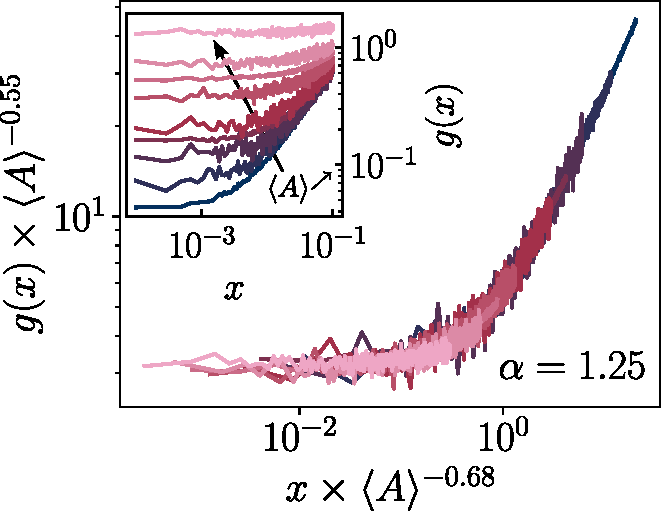
\includegraphics[width=0.45\textwidth]{Chapitre3/Figures/Interpretation/PCorr/PCorr_rescaled_alpha125_mean.pdf}
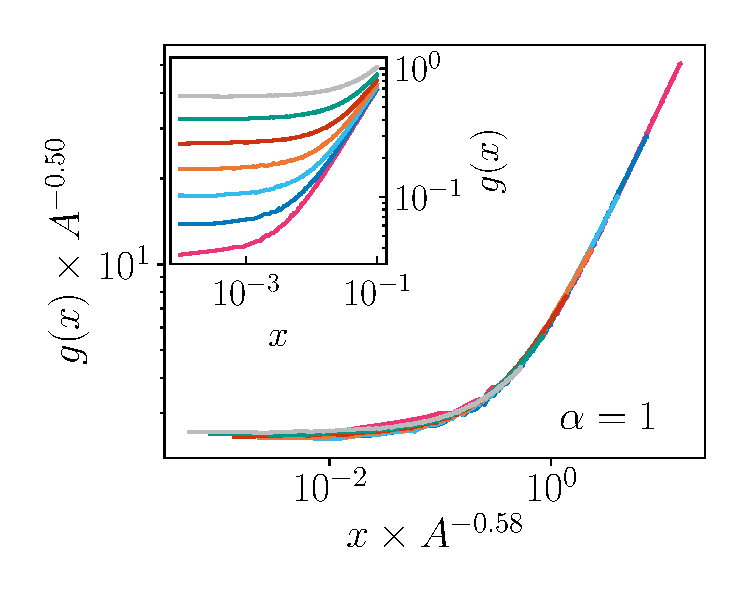
\includegraphics[width=0.45\textwidth]{Chapitre3/Figures/Interpretation/PCorr/PCorr_rescaled_alpha1_mean.pdf}
\caption{Idem que pour la \autoref{fig:PCorr_alpha} pour $\alpha = 1.25$ (gauche) et $\alpha = 1$ (droite)}
\label{fig:PCorrAnnexe5}
\end{figure}

\begin{figure}[h]
\centering
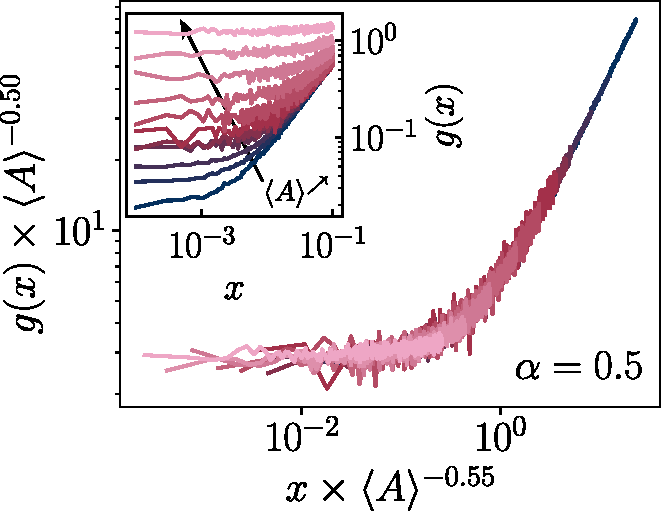
\includegraphics[width=0.45\textwidth]{Chapitre3/Figures/Interpretation/PCorr/PCorr_rescaled_alpha05_mean.pdf}
\caption{Idem que pour la \autoref{fig:PCorr_alpha} pour $\alpha = 0.5$}
\label{fig:PCorrAnnexe5}
\end{figure}

\FloatBarrier

\section{Avalanches dans le modèle $\alpha$-ROM}

\label{sec:AvTBLRRAnnexe}

\begin{figure}[h]
\centering
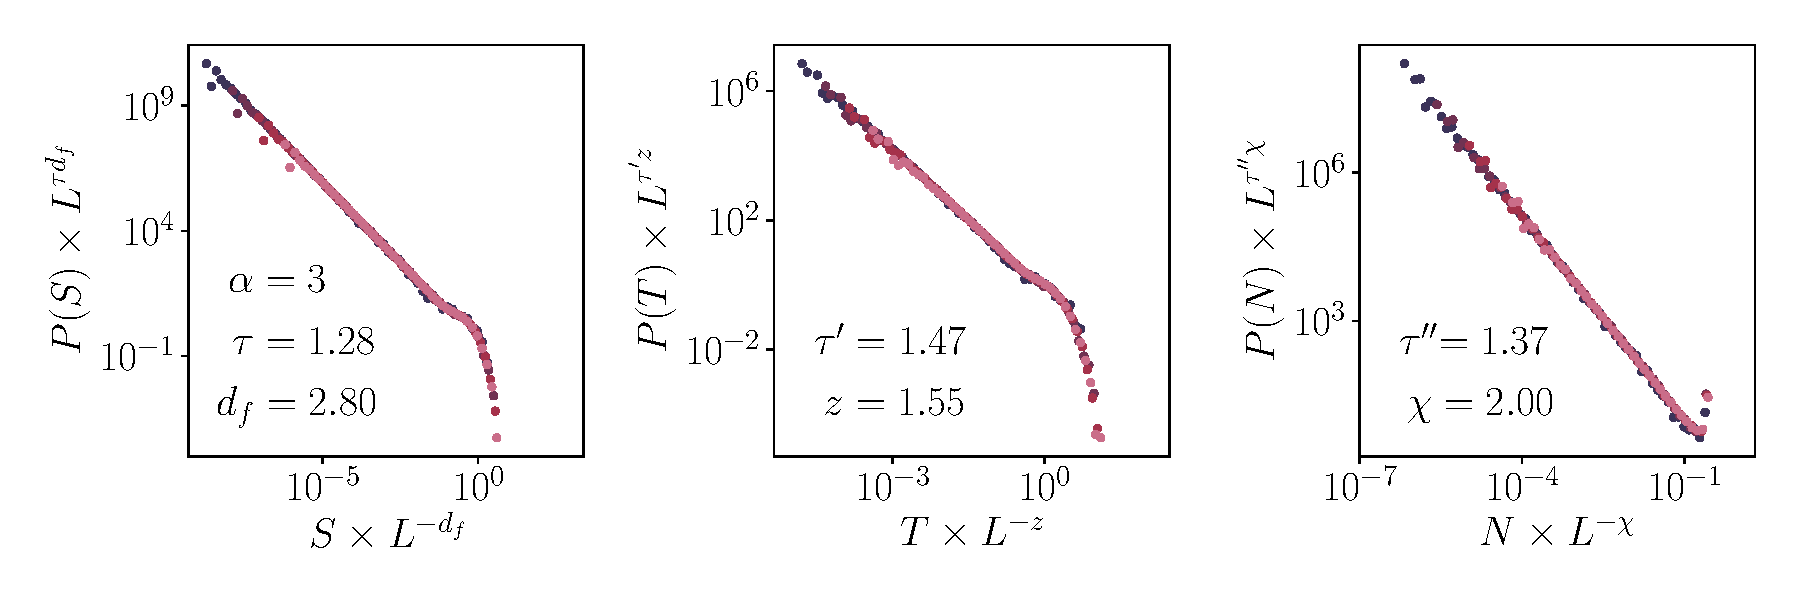
\includegraphics[width=\textwidth]{Chapitre3/Figures/Avalanches/Rescale_Av_alpha3.pdf}
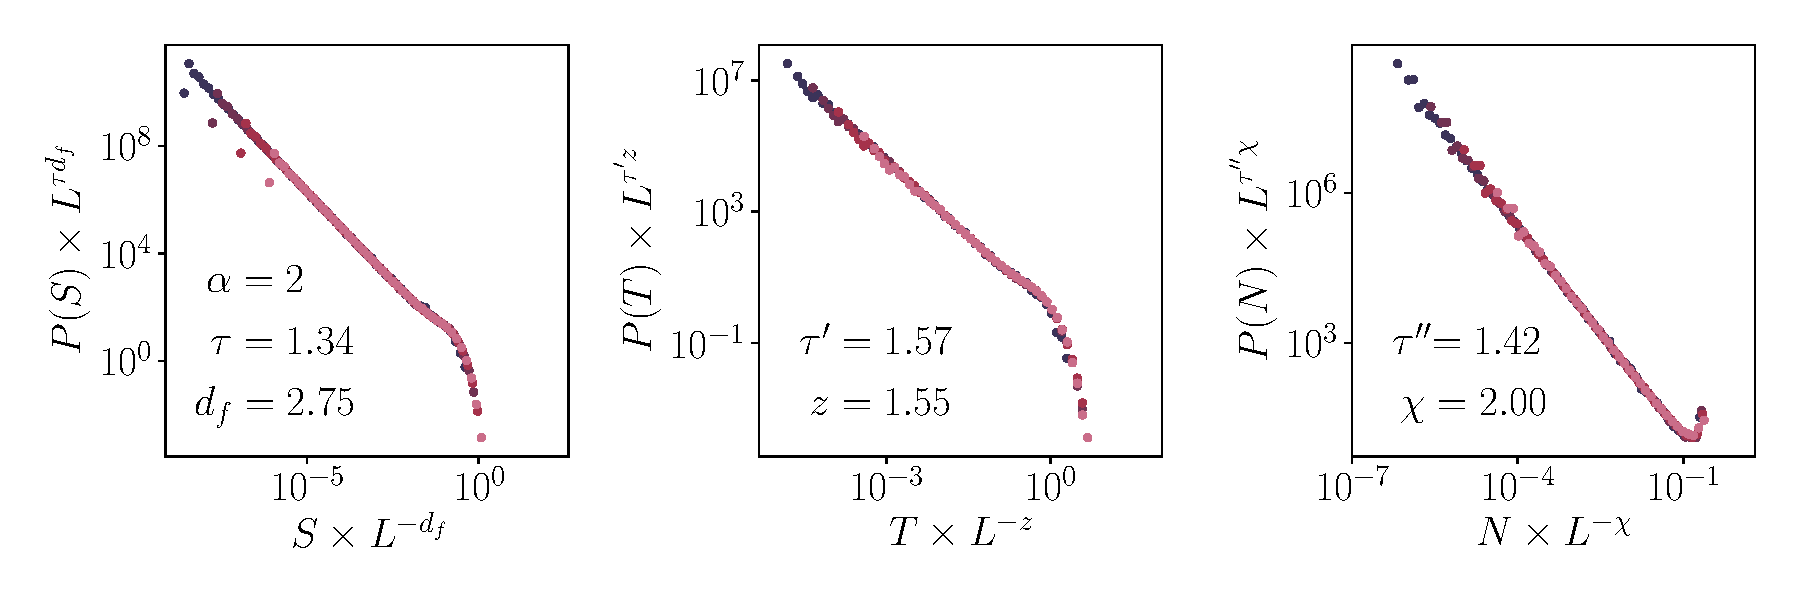
\includegraphics[width=\textwidth]{Chapitre3/Figures/Avalanches/Rescale_Av_alpha2.pdf}
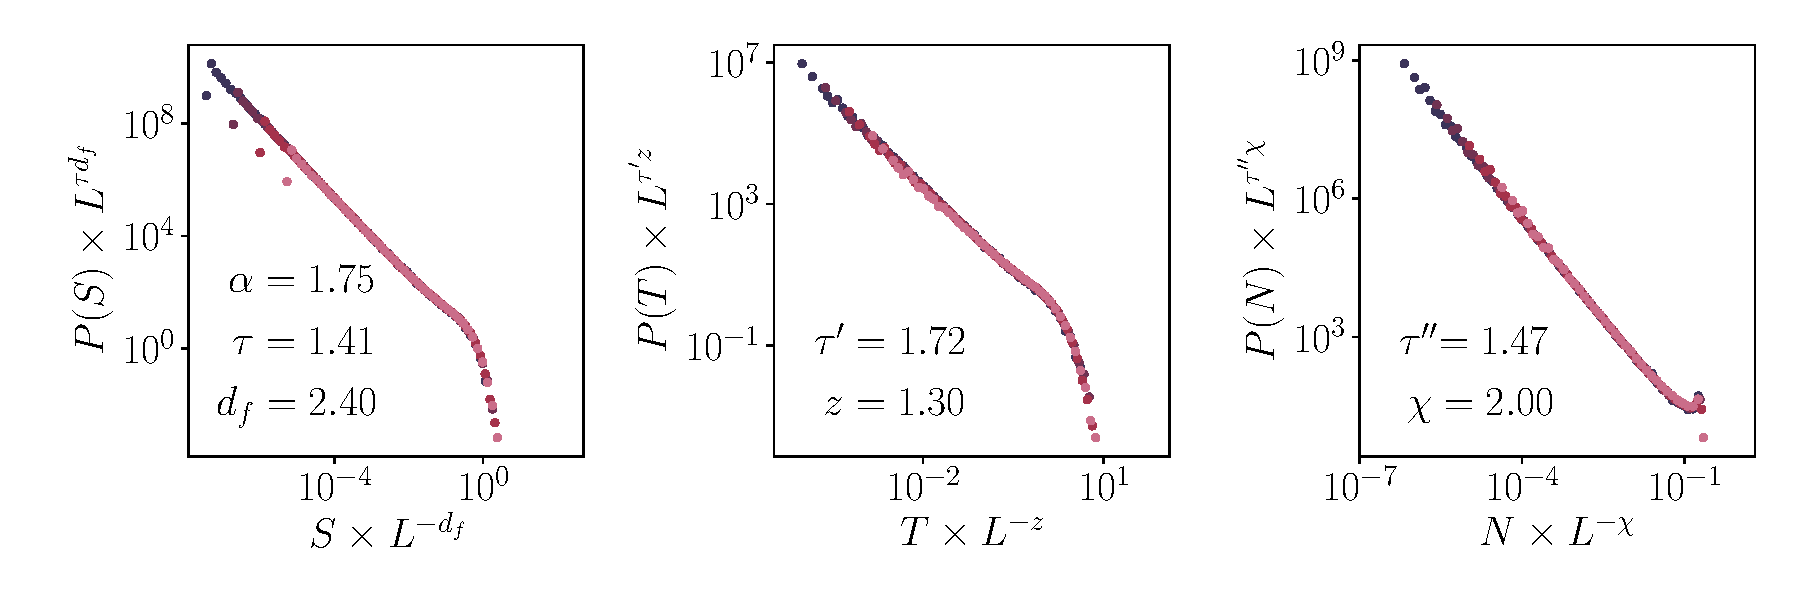
\includegraphics[width=\textwidth]{Chapitre3/Figures/Avalanches/Rescale_Av_alpha175.pdf}
\caption{}
\label{fig:annexeAvTBLRR1}
\end{figure}

\begin{figure}[h]
\centering
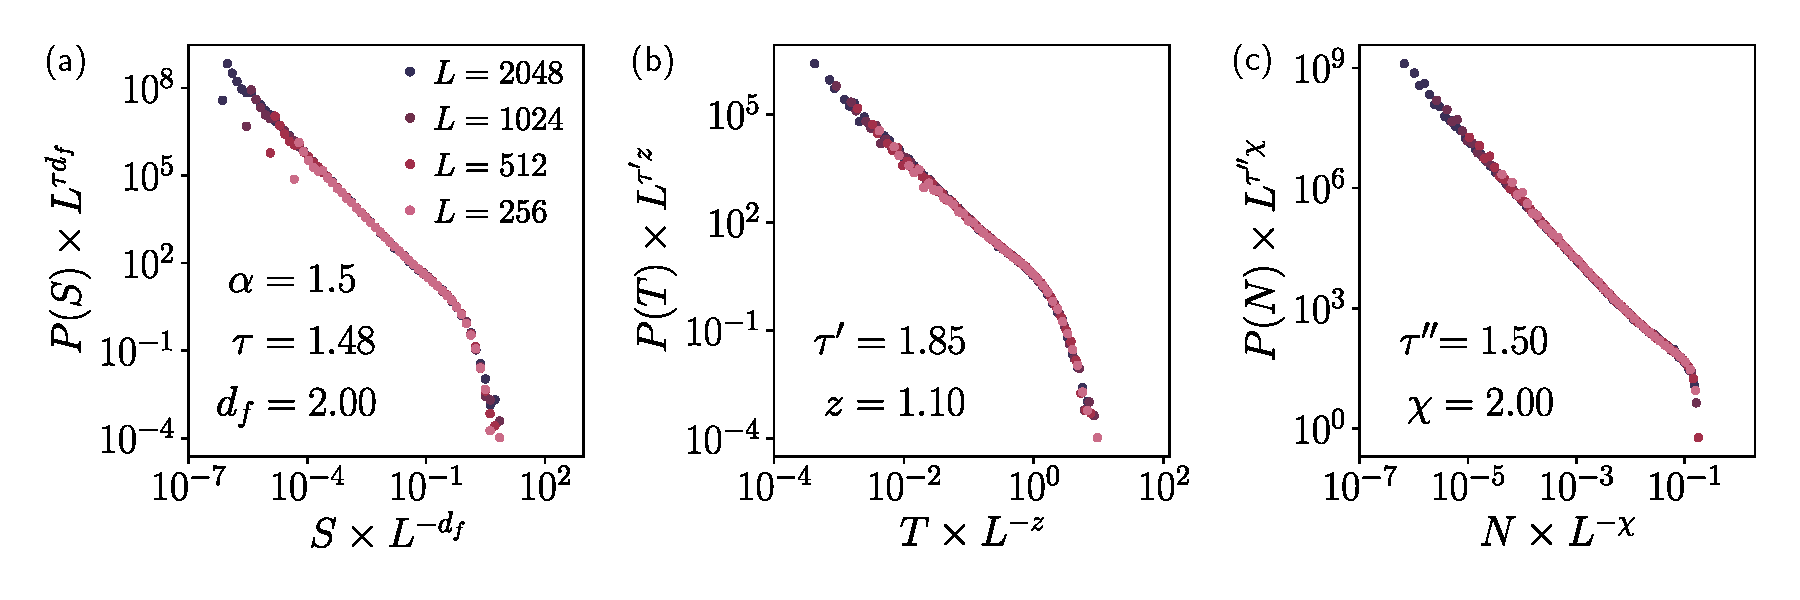
\includegraphics[width=\textwidth]{Chapitre3/Figures/Avalanches/Rescale_Av_alpha15.pdf}
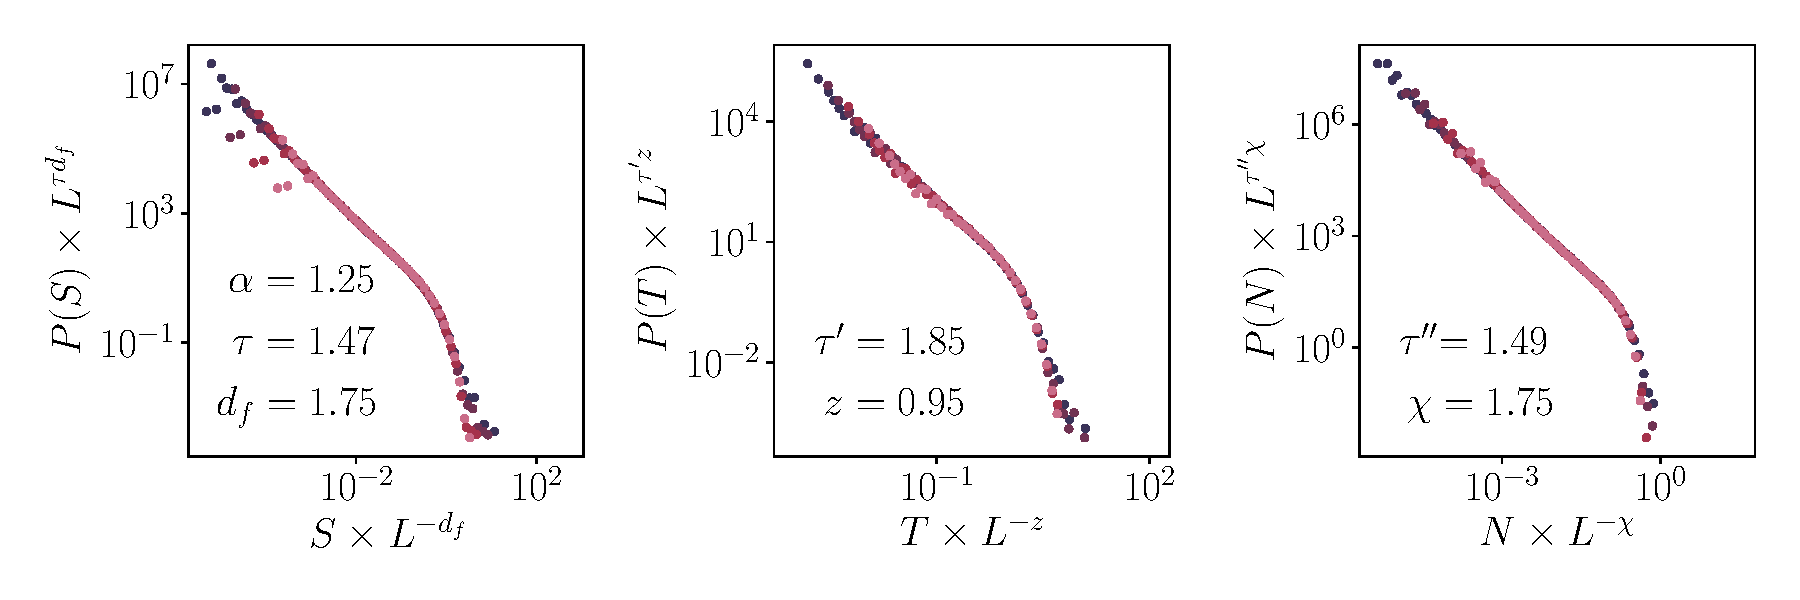
\includegraphics[width=\textwidth]{Chapitre3/Figures/Avalanches/Rescale_Av_alpha125.pdf}
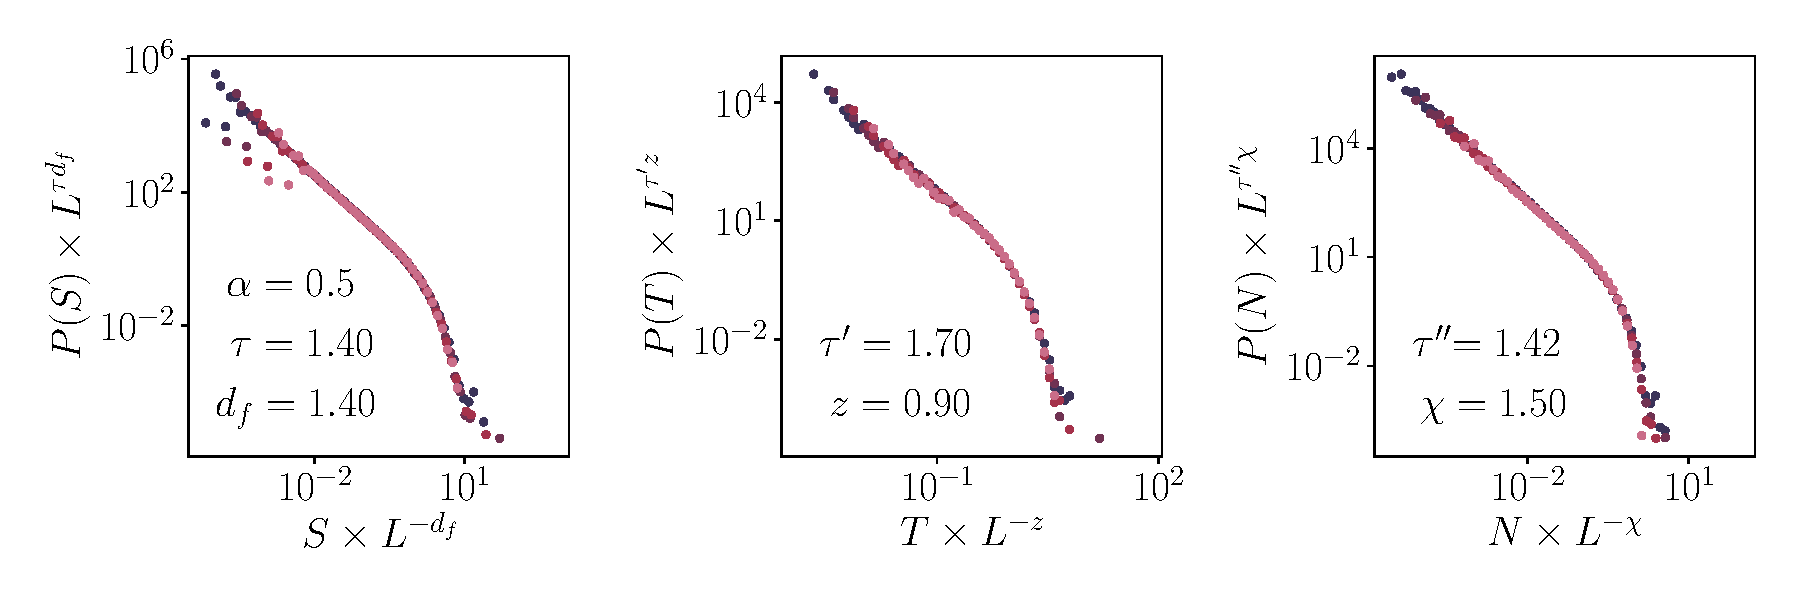
\includegraphics[width=\textwidth]{Chapitre3/Figures/Avalanches/Rescale_Av_alpha05.pdf}
\caption{}
\label{fig:annexeAvTBLRR2}
\end{figure}

\FloatBarrier

\chapter{Annexes au chapitre 4}



\section{Modèles $\alpha$-Picard}

\subsection{Transformée de Fourier inverse du propagateur}

\label{sec:TFinverse}

\subparagraph{}Dans cette partie, nous faisons le lien entre les formes spectrales des propagateurs dans les modèles $\alpha$-Picard présentées au \autoref{chapter:yielding} et leur forme dans l'espace réel. Pour ce faire, nous cherchons la transformée de Fourier inverse en 2D en espace continue de la fonction :

\begin{equation}
	f(\mathbf{q}) = \frac{q_x^2 q_y^2}{q^{6-\alpha}}
\end{equation}

\noindent et nous notons $\beta = 6 - \alpha$ pour simplifier les notations dans le calcul qui suit.

\paragraph{}Nous commençons par partir du résultat général :

\begin{equation}
    \mathcal{F}\left( \frac{1}{r^\alpha} \right)=\frac{\pi^{\alpha-d / 2} \Gamma((d-\alpha) / 2)}{\Gamma(\alpha / 2)} \times\frac{1}{|k|^{d-\alpha}}
\end{equation}

\noindent avec $\mathbf{q} = 2\pi \mathbf{k}$ et $d$ la dimension de l'espace. Ce résultat est valable pour $0<\alpha<d$ dans le sens des fonctions mais peut être étendu à tout $\alpha$ au sens des distributions. De manière équivalente nous avons donc :

\begin{equation}
    \mathcal{F}^{-1}\left( \frac{1}{\lvert k \rvert^\beta} \right) = \frac{\Gamma\left( 1-\frac{\beta}{2} \right)}{\pi^{1-\beta}\Gamma\left( \frac{\beta}{2} \right)}\times\frac{1}{r^{2-\beta}}
\end{equation}

\noindent et donc :

\begin{equation}
\begin{aligned}
    (2\pi)^4\mathcal{F}^{-1}\left( \frac{k_x^2k_y^2}{\lvert k \rvert^\beta} \right) &= \partial_x^2\partial_y^2\mathcal{F}^{-1}\left( \frac{1}{\lvert k \rvert^\beta} \right)\\
    &=\frac{\Gamma\left( 1-\frac{\beta}{2} \right)}{\pi^{1-\beta}\Gamma\left( \frac{\beta}{2} \right)}\partial_x^2\partial_y^2\left( \frac{1}{r^{2-\beta}} \right)
\end{aligned}
\end{equation}

\noindent Le calcul des dérivées donne :

\begin{equation}
    \partial_x^2\partial_y^2\left( \frac{1}{r^{2-\beta}} \right) = \frac{1}{r^{10-\beta}}(8-6\beta+\beta^2)\times\left(x^4(\beta-5)+y^4(\beta-5)+x^2y^2(38-12\beta+\beta^2)\right)
\end{equation}

\noindent et nous pouvons simplifier cette expression en utilisant  $r^2=x^2+y^2$ et $(x,y)=(r\cos\theta,r\sin\theta)$ selon :

\begin{equation}
    \partial_x^2\partial_y^2\left( \frac{1}{r^{2-\beta}} \right) = \frac{1}{r^{6-\beta}}(8-6\beta+\beta^2)\times\left(\beta-5+\cos^2\theta\sin^2\theta(48-14\beta+\beta^2)\right)
\end{equation}

\noindent puis en utilisant la relation trigonométrique $\cos^2\theta\sin^2\theta = \frac{1}{8}(1-\cos4\theta)$ on a :

\begin{equation}
    \partial_x^2\partial_y^2\left( \frac{1}{r^{2-\beta}} \right) = \frac{1}{8r^{6-\beta}}(8-6\beta+\beta^2)\times\left((8-6\beta+\beta^2)-\cos4\theta(48-14\beta+\beta^2)\right)
\end{equation}

\noindent et donc en factorisant on a finalement :

\begin{equation}
    (2\pi)^4\mathcal{F}^{-1}\left( \frac{k_x^2k_y^2}{\lvert k \rvert^\beta} \right) = \frac{\Gamma\left( 1-\frac{\beta}{2} \right)}{\pi^{1-\beta}\Gamma\left( \frac{\beta}{2} \right)}\times\frac{(\beta-4)(\beta-2)}{8r^{6-\beta}}\left( (\beta-4)(\beta-2)-\cos4\theta(\beta-8)(\beta-6) \right)
\end{equation}

\noindent soit :

\begin{equation}
    \mathcal{F}^{-1}\left( \frac{q_x^2q_y^2}{\lvert q \rvert^\beta} \right) = \frac{\Gamma\left( 1-\frac{\beta}{2} \right)}{\pi 2^\beta\Gamma\left( \frac{\beta}{2} \right)}\times\frac{(\beta-4)(\beta-2)}{8r^{6-\beta}}\left( (\beta-4)(\beta-2)-\cos4\theta(\beta-8)(\beta-6) \right)
\end{equation}

\noindent ce qui permet de retrouver la forme donnée à l'\autoref{eq:RealAlphaPicard}.


\paragraph{Développement autour de $\beta = 4$/$\alpha=2$}

\subparagraph{}Les entiers négatifs (zéro inclut) sont des pôles de la fonction $\Gamma$. Le cas $\beta = 4$ correspondant au propagateur d'Eshelby doit être pris comme une limite. Pour ce faire, nous utilisons le développement :

\begin{equation}
    \Gamma(-n+\epsilon) = \frac{(-1)^n}{n!}\left( \frac{1}{\epsilon}+\mathcal{O}(1) \right)
\end{equation}

\noindent qui nous permet donc d'obtenir pour $\beta=4+\epsilon$ :

\begin{equation}
    (2\pi)^4\mathcal{F}^{-1}\left( \frac{k_x^2k_y^2}{\lvert k \rvert^{4+\epsilon}} \right)=\frac{2/\epsilon}{\pi^{-3-\epsilon/2}\Gamma\left( 2+\frac{\epsilon}{2} \right)}\times\frac{(\epsilon+2)\epsilon}{8r^{2-\epsilon}}((\epsilon+2)\epsilon-\cos4\theta(\epsilon-2)(\epsilon-4))
\end{equation}

\noindent qui permet d'arriver dans la limite $\epsilon \rightarrow 0$ à :

\begin{equation}
    \mathcal{F}^{-1}\left( \frac{-4q_x^2q_y^2}{\lvert q \rvert^{4}} \right)=\frac{\cos4\theta}{\pi r^2}
\end{equation}

\subsection{Détermination des points critiques}

\label{sec:CP_aPicard}

\subparagraph{}Dans cette partie, nous présentons simplement sur la \autoref{fig:CP_aPicard} les données ayant permis la détermination des contraintes critiques $\Sigma_c$ et de l'exposant $\beta$ pour chaque déclinaison du modèle $\alpha$-Picard. La détermination est réalisée à contrainte imposée, de la même manière que pour les modèles d'écoulement de courte portée Picard-CP et FES$^\pm$.

\begin{figure}[H]
	\centering
	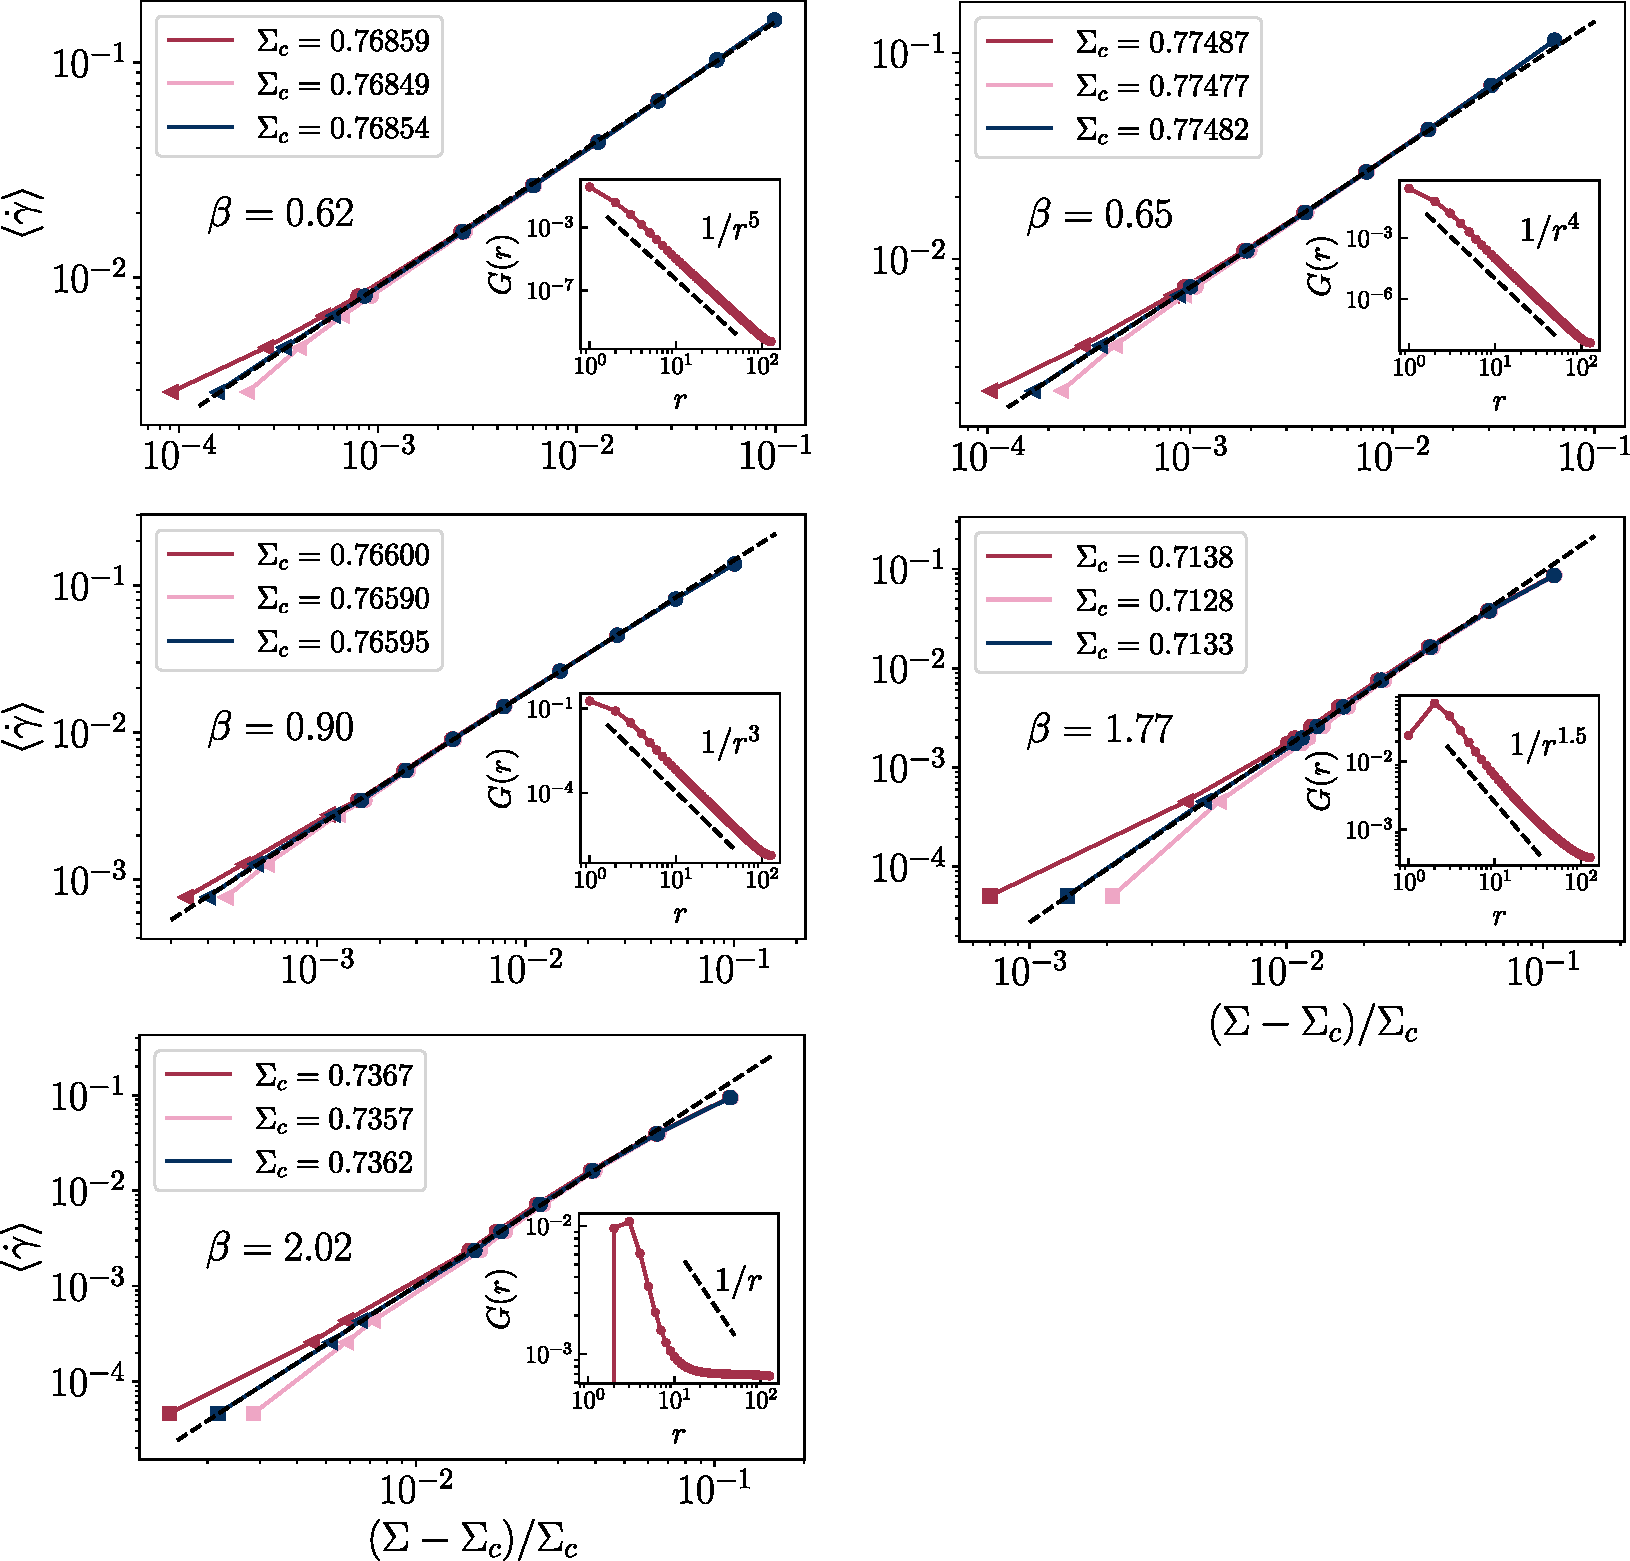
\includegraphics[width=\textwidth]{Chapitre6/Figures/CP_alphaPicard.pdf}
	\label{fig:CP_aPicard}
	\caption{Détermination de la contrainte critique $\Sigma_c$ et de l'exposant $\beta$ pour les modèles $\alpha$-Picard avec $\alpha \in \{ 5, 4, 3, 1.5, 1 \}$. En encart, la forme du propagateur dans l'espace réel implémenté de la façon présentée à la \autoref{sec:alphaPicard}}
\end{figure}

\subsection{Avalanches}

\subparagraph{}Dans cette partie, nous présentons à la \autoref{fig:Av_rescale_alpha_annexe} les données utilisées pour la caractérisation des avalanches à contrainte imposée dans les modèles $\alpha$-Picard pour les portées non présentées au \autoref{chapter:yielding}. Le protocole utilisé est celui présenté à la \autoref{sec:Av_PicardMain}.

\begin{figure}[H]
	\centering
	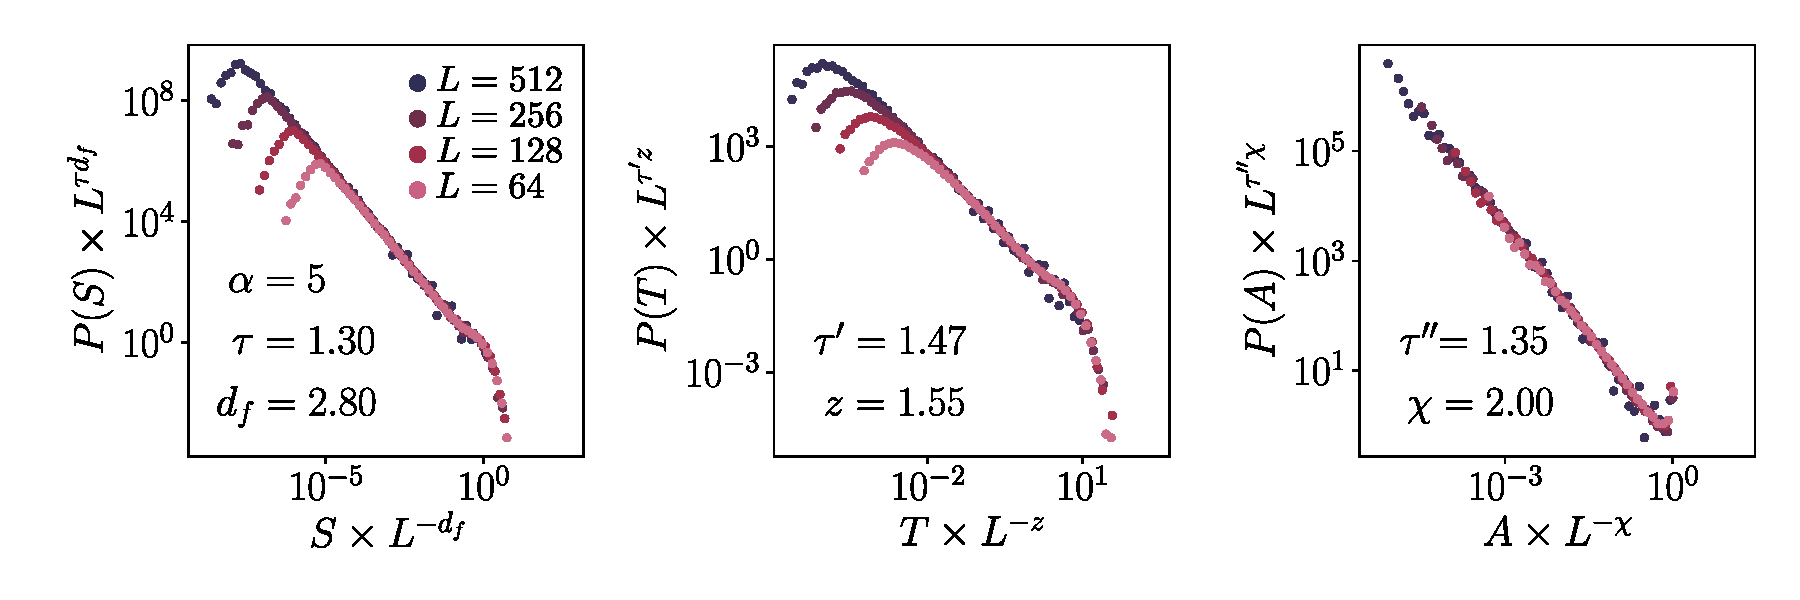
\includegraphics[width=\textwidth]{Chapitre4/Figures/Avalanches/Rescale_Av_alpha5.pdf}
	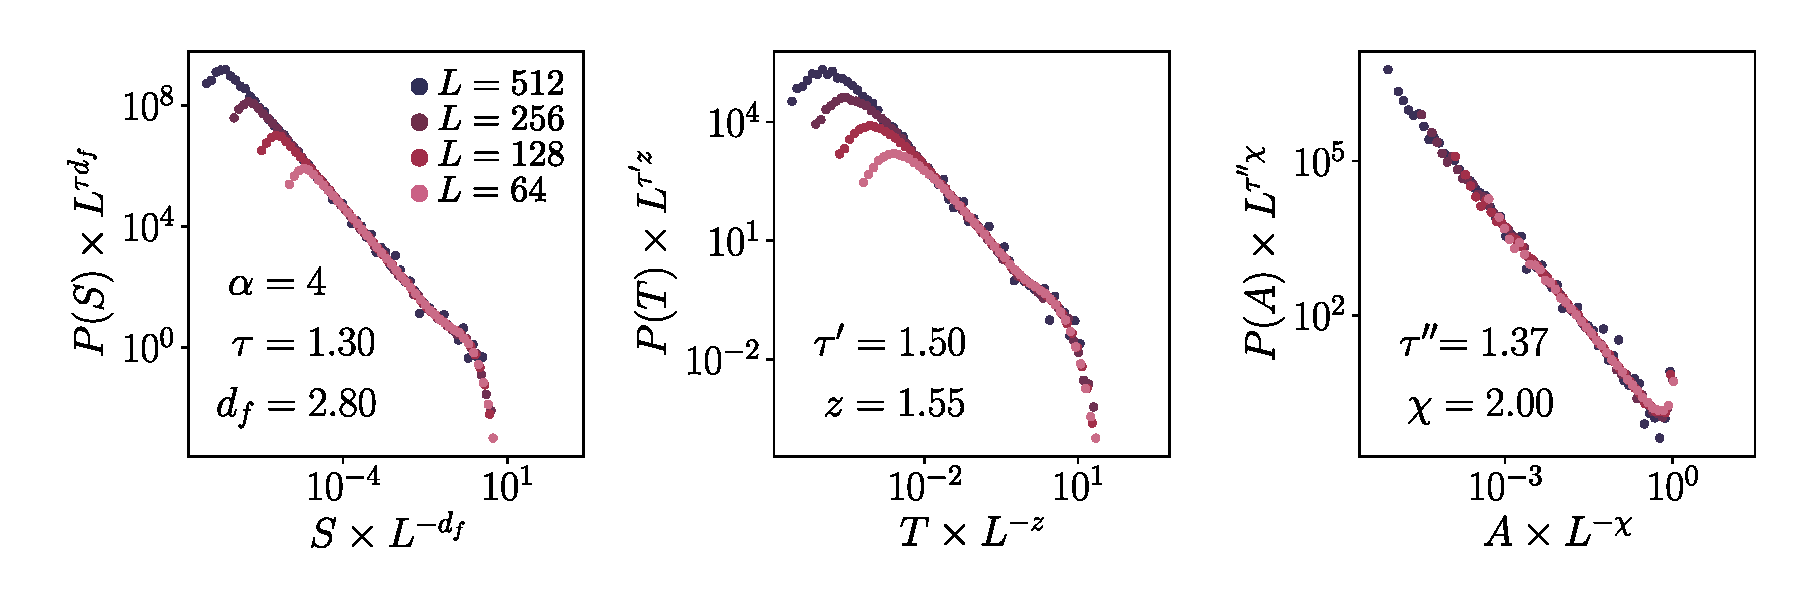
\includegraphics[width=\textwidth]{Chapitre4/Figures/Avalanches/Rescale_Av_alpha4.pdf}
	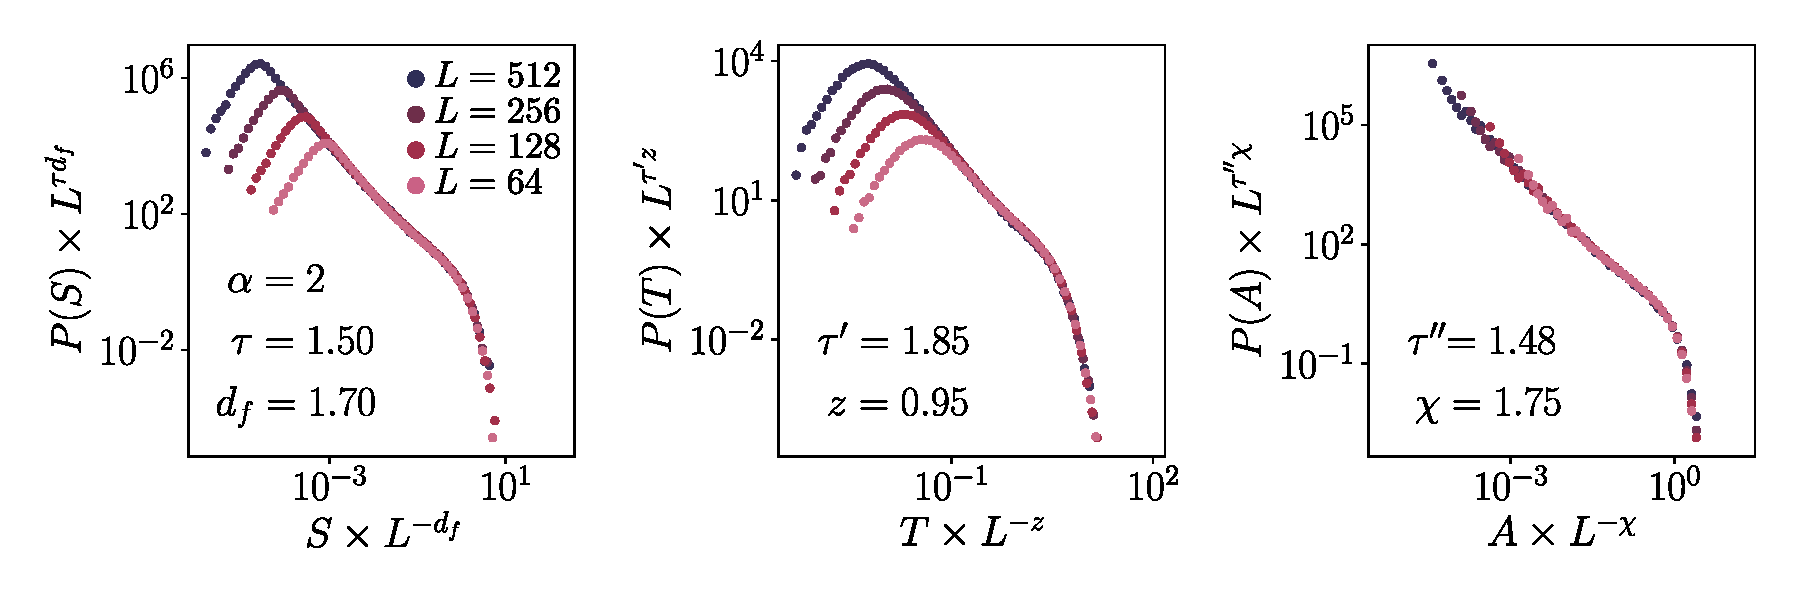
\includegraphics[width=\textwidth]{Chapitre4/Figures/Avalanches/Rescale_Av_alpha2.pdf}
	\caption{Distributions de tailles (a), de durées (b) et de surfaces (c) d'avalanche redimensionnées dans le modèle $\alpha$-Picard pour $\alpha \in \{5, 4, 2 \}$.}
	\label{fig:Av_rescale_alpha_annexe}
\end{figure}

\section{Dépendance en protocole des avalanches à contrainte imposée dans les modèles élastoplastiques}

\label{sec:article2}

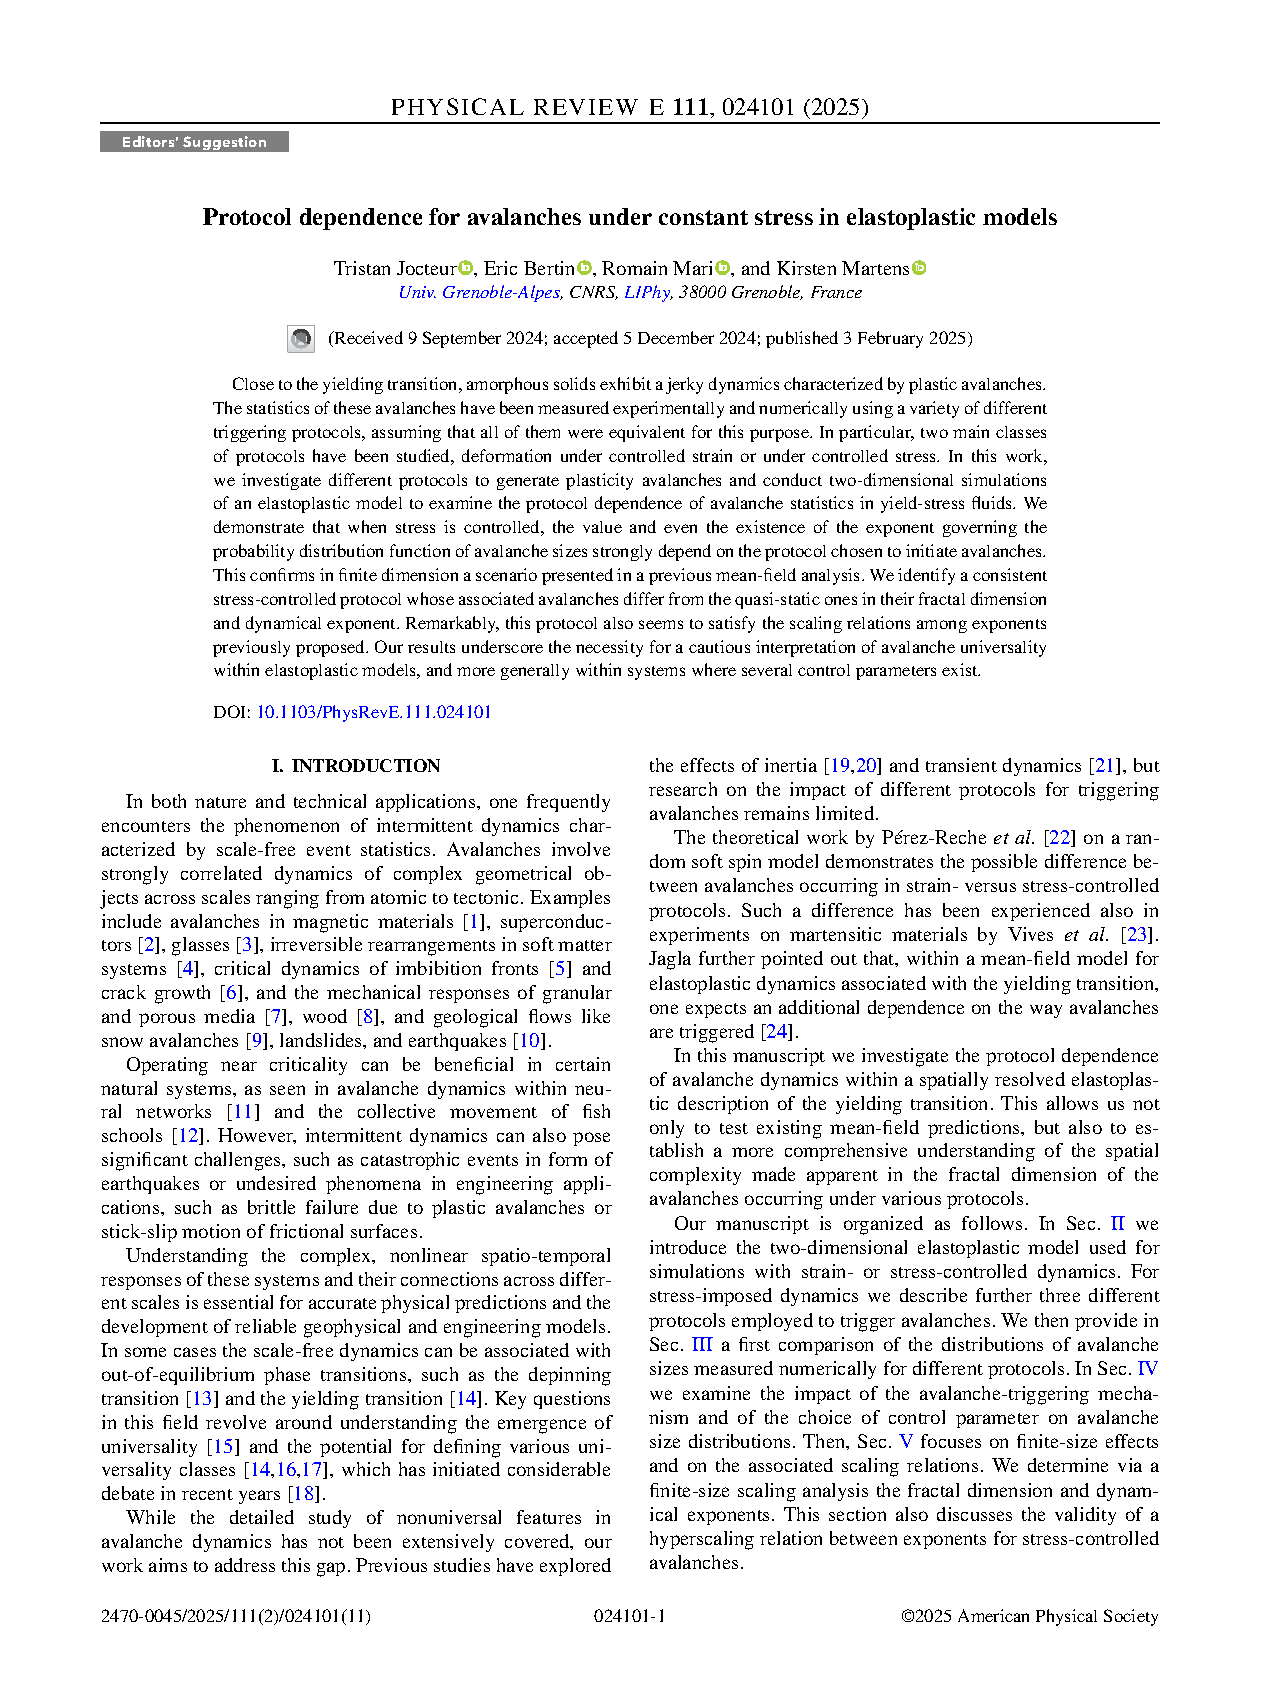
\includepdf[noautoscale=true, width=\paperwidth, pages=-]{PhysRevE.111.024101.pdf}

\section{Modèle de Picard confiné}

\label{sec:lambda_picard}

\subparagraph{}Dans cette partie nous présentons une très brève étude de la transition vers l'écoulement dans un dispositif quasi-2D représentant un confinement entre deux plaques rigides. Pour ce faire, nous commençons par exposer la modification du propagateur de redistribution de la contrainte locale dans ce cas. Puis, via son analyse dans le cadre du modèle de Picard, nous montrons que cette nouvelle forme de l'interaction, toujours à longue portée, induit une perte de criticalité au-delà d'une certaine longueur d'écrantage définie par le confinement.

\subsection{Confinement et interaction d'Eshelby}

\subparagraph{}De la même façon que dans le cas des suspensions, les dispositifs expérimentaux étudiés dans le cas de la transition vers l'écoulement peuvent agir significativement sur la portée des interactions. Si le cas de l'interaction d'Eshelby est le plus plébiscité dans la communauté des matériaux amorphes, nous pouvons imaginer une variation de la modification de contrainte induite par un réarrangement plastique dans un dispositif différent. En effet, si l'on considère un écoulement quasi-2D dans le plan $(\hat{\mathbf{e}}_x, \hat{\mathbf{e}}_y)$ entre deux plaques rigides parallèles aux plans de côte $z$ constante, alors les frottements entre le fluide à seuil s'écoulant et les plaques vont induire une dissipation modifiant la redistribution de contrainte suite à un évènement plastique. 

\subparagraph{}Pour le comprendre, nous proposons modéliser ces frottements par un terme de dissipation proportionnel à la défomation du fluide de la même manière que dans le cas de l'étude des écoulements en milieux poreux \cite{long_note_2001}. Dans ce cadre, la condition d'équilibre mécanique dans l'espace 2D effectif devient (voir \autoref{sec:Annexe_Eshelby}) :

\begin{equation}
	-\partial_i P^1(\mathbf{r}) + \partial_j\sigma_{ij}^1(\mathbf{r}) - \mu\lambda^2 u^1_{i}= 0
\end{equation}

\noindent avec $\lambda$ un coefficient retranscrivant l'intensité de la dissipation et définissant une longueur d'écrantage $\xi \sim 1/\lambda$. Par une résolution similaire à celle présentée dans la \autoref{sec:Annexe_Eshelby}, ce cas de figure nous amène à un propagateur dans l'espace réciproque dont la forme est la suivante :

\begin{equation}
    \hat{G}_\lambda(\mathbf{q}) = -4\frac{q_x^2q_y^2}{q^2(q^2+\lambda^2)}-\frac{\lambda^2}{\lambda^2+q^2}
    \label{eq:screenedEshelby}
\end{equation}

\noindent et dont on peut déterminer les formes asymptotiques en se basant sur la forme dans l'espace réel des propagateurs des modèles $\alpha$-Picard :

\begin{equation}
\begin{aligned}
    \hat{G}_\lambda(\mathbf{q})\xrightarrow[q\gg \lambda]{}-4\frac{q_x^2q_y^2}{q^4} \quad &\Rightarrow \quad G_\lambda(\mathbf{r})\xrightarrow[r\ll \xi]{}\sim\frac{\cos 4\theta}{r^2}\\
    \hat{G}_\lambda(\mathbf{q})\xrightarrow[q \ll \lambda]{}-4\frac{q_x^2q_y^2}{\lambda^2 q^2}-1 \quad &\Rightarrow \quad G_\lambda(\mathbf{r})\xrightarrow[r \gg \xi]{}\sim\frac{\cos 4\theta}{r^4}
\end{aligned}
\end{equation}

\noindent Ainsi, dans l'espace réel, en dehors de la relaxation globale imposée par le terme de dissipation, la redistribution du système confiné est la même que celle dans le problème original à petite distance $r\ll \xi$, décroissant comme $\sim 1/r^2$, mais, au-delà de la longueur d'écrantage, celle-ci décroît significativement plus vite, comme $\sim 1/r^4$. Ainsi, comme dans le cas des suspensions, le confinement ne supprime pas le caractère de longue portée de l'interaction mais change son évolution algébrique.

\paragraph{Transformée de Fourier inverse du propagateur}

\subparagraph{}Pour obtenir l'expression complète du propagateur en espace réel, nous pouvons décomposer le premier terme de l'\autoref{eq:screenedEshelby} de la manière suivante :

\begin{equation}
    \hat{G}_\lambda(\mathbf{q}) = -4\frac{q_x^2q_y^2}{\lambda^2 q^2} + 4\frac{q_x^2q_y^2}{\lambda^2 (\lambda^2 + q^2)}-\frac{\lambda^2}{\lambda^2+q^2}
\end{equation}

\noindent pour obtenir dans l'espace réel :

\begin{equation}
    G(r,\theta) = \frac{12}{\pi\lambda^2}\frac{\cos 4\theta}{r^4}-\frac{\lambda^2}{2\pi}K_0(\lambda r)+\frac{2}{\pi\lambda^2}\partial_x^2\partial_y^2K_0(\lambda r)
\end{equation}

\noindent En calculant les dérivées associées au troisème terme du membre de droite, nous obtenons donc :

\begin{equation}
    G(r,\theta) = \frac{12}{\pi\lambda^2}\frac{\cos 4\theta}{r^4} - \frac{1}{32\pi\lambda r^3}\sum_{n=0}^{4}K_n(\lambda r)\left(P_n^{(0)}(\lambda r) + P_n^{(1)}(\lambda r)\cos 4\theta\right)
\end{equation}

\noindent avec :

\begin{equation}
    \begin{aligned}
        &P_0^{(0)}(X) = X(4+13X^2), \quad &P_0^{(1)}(X) = 3X(20+X^2)\\
        &P_1^{(0)}(X) = 8+12X^2,\quad &P_1^{(1)}(X) = 120+36X^2\\
        &P_2^{(0)}(X) = 4X(1-X^2),\quad &P_2^{(1)}(X) = 60X^3\\
        &P_3^{(0)}(X) = 4X^2,\quad &P_3^{(1)}(X) = 12X^2\\
        &P_4^{(0)}(X) = -X^3,\quad &P_4^{(1)}(X) = X^3\\
    \end{aligned}
\end{equation}

\subsection{Etude des avalanches dans le modèle $\lambda$-Picard}

\label{sec:screenedav}

\subparagraph{}Pour étudier la transition vers l'écoulement dans un dispositif confiné quasi-2D, nous implémentons la forme du propagateur donnée par l'\autoref{eq:screenedEshelby} dans le modèle de Picard de la même façon que dans le cas du modèle $\alpha$-Picard. Ce modèle dépend d'un paramètre continu $\lambda$ et nous le baptisons alors modèle $\lambda$-Picard. Via cette implémentation, nous obtenons les formes de décroissance du propagateur représentées à la \autoref{fig:screenedprop} et compatibles avec les comportements asymptotiques en $\sim 1/r^2$ et en $\sim 1/r^4$.

\begin{figure}[h]
	\centering
	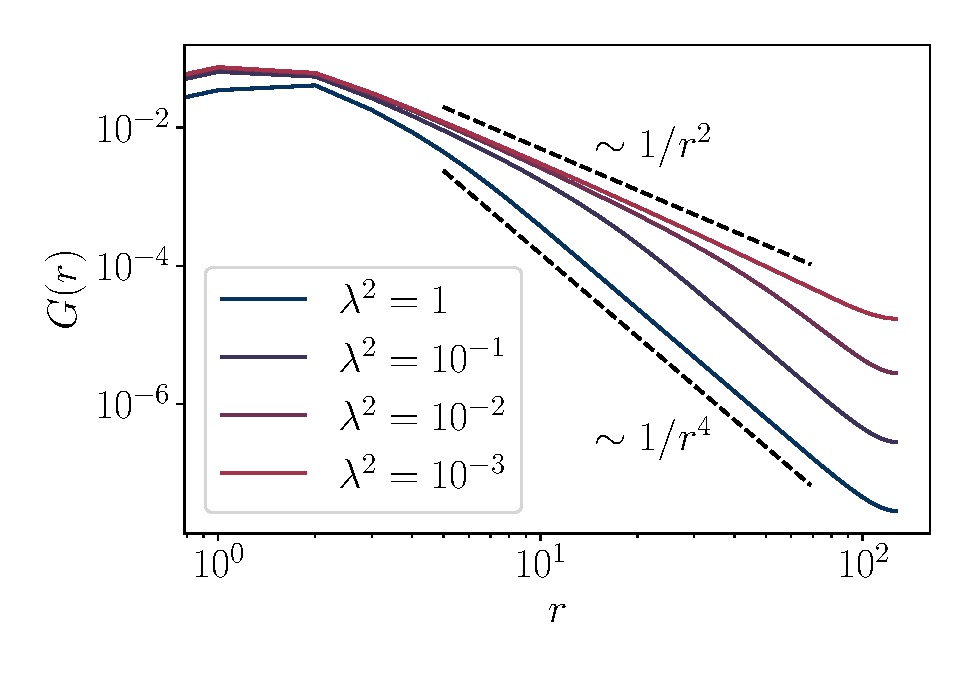
\includegraphics[width=0.6\textwidth]{Chapitre6/Figures/ScreenedPropagators.pdf}
	\caption{Images des propagateurs de redistribution dans le modèle $\lambda$-Picard. La figure montre l'évolution du propagateur le long de la ligne $y=0$ pour différentes valeurs d'écrantage $\lambda$.}
	\label{fig:screenedprop}
\end{figure}

\subparagraph{}Le modèle de Picard confiné ne conservant pas la contrainte globale du système, il n'est pas possible de générer des avalanches selon le protocole de contrainte imposée RTP (voir \autoref{sec:AvYielding}). Toutefois, l'approche quasistatique de l'AQS est tout à fait réalisable. Pour différentes tailles de systèmes $L$ et différents écrantages $\lambda$, nous mesurons donc les distributions de tailles d'avalanche avec le protocole AQS dans ce modèle. Les résultats sont présentés à la \autoref{fig:EvolLambdaAv}.

\begin{figure}[h]
	\centering
	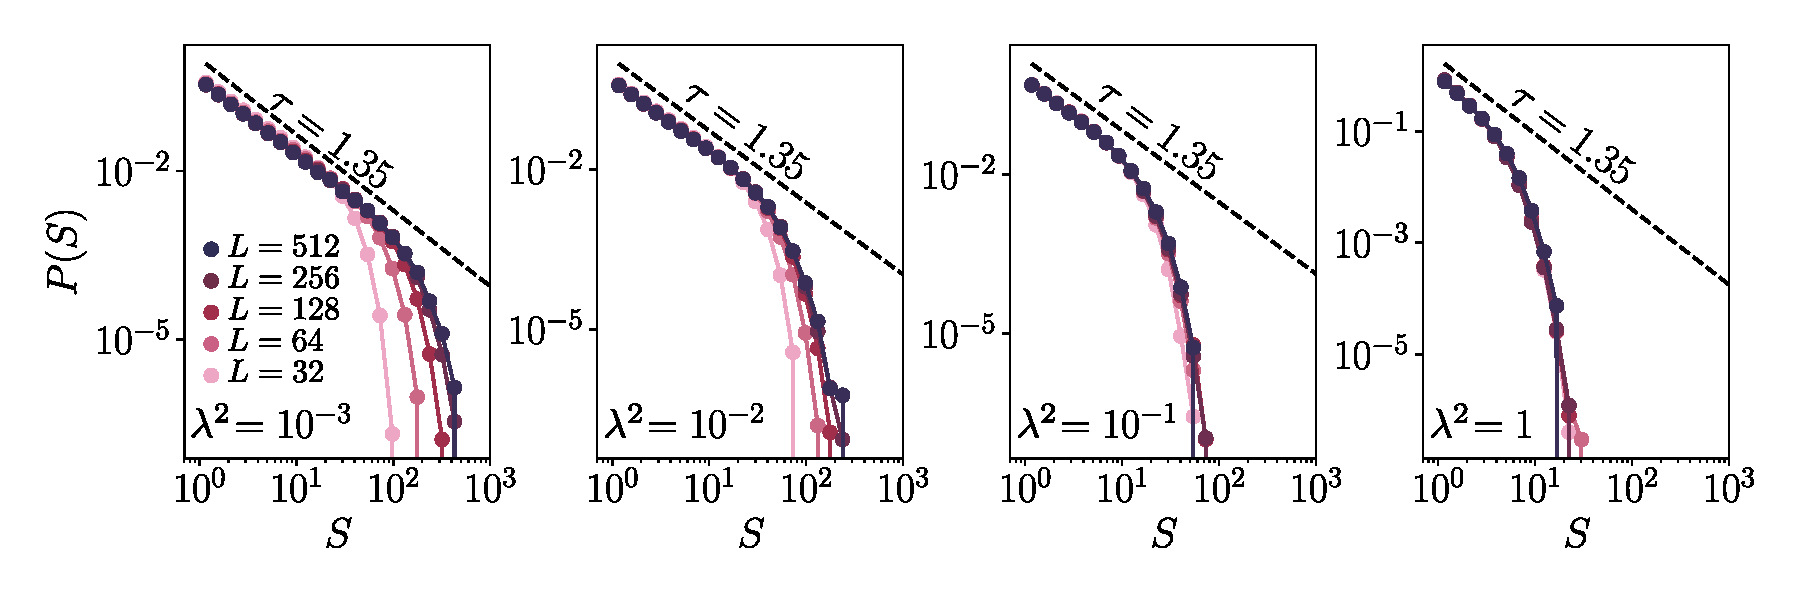
\includegraphics[width=\textwidth]{Chapitre4/Figures/Avalanches/EvolLambdaAv.pdf}
	\label{fig:EvolLambdaAv}
	\caption{Distributions de tailles d'avalanche quasistatiques dans le modèle de Picard écranté pour différentes valeurs de l'écrantage $\lambda$}
\end{figure}

\subparagraph{}Pour le plus faible écrantage ($\lambda^2 = 10^{-3}$), nous retrouvons des distributions en loi de puissance avec $\tau \approx 1.35$ comme dans le cas du modèle de Picard ($\lambda = 0$). Par contre, à mesure que $\lambda$ augmente, ces lois de puissance montrent un cut-off $S_c(\lambda)$ diminuant peu à peu. De ce fait, à $\lambda=1$ la criticalité avalancheuse est perdue à toutes les tailles. Cette diminution du cut-off ne dépendant pas de la taille du système, cela suggère qu'il est uniquement contrôlé par la longueur d'écrantage $\xi \sim 1/\sqrt{\lambda}$. En d'autres termes, il n'y aurait des avalanches qu'en dessous de la longueur d'écrantage. Au-delà, le système perd sa criticalité. Etant donné qu'en dessous de $\xi$ le propagateur prend la forme de celui du propagateur d'Eshelby, il est raisonnable de penser que les avalanches ont la même structure que celles dans le modèle de Picard dans la zone non-écrantée. Pour valider cette hypothèse, nous redimensionnons les distributions obtenues pour les systèmes de plus grande taille ($L=512$) selon :

\begin{equation}
	P(S) \rightarrow \frac{P(S)}{\xi^{-\tau_\text{eff}d_{f,\text{eff}}}},\quad S\rightarrow \frac{S}{\xi^{d_{f,\text{eff}}}}, \quad \xi = \frac{1}{\lambda}
\end{equation}

\begin{figure}[h]
	\centering
	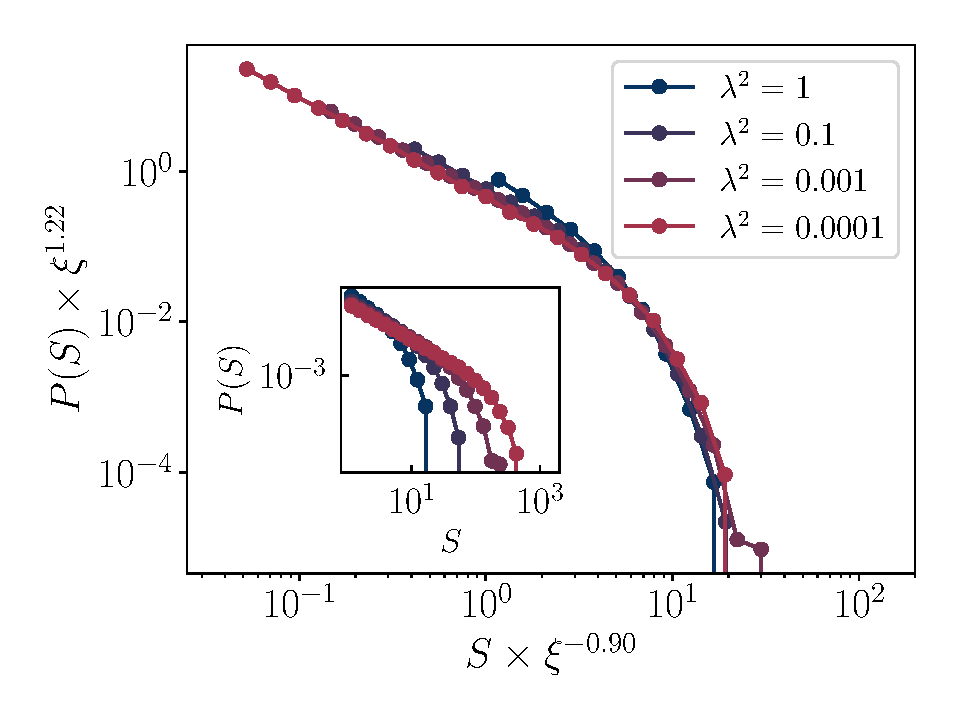
\includegraphics[width=0.65\textwidth]{Chapitre6/Figures/RescaleScreenedAv.pdf}
	\label{fig:RescaleScreenedAv}
	\caption{Redimensionnement des distributions de tailles d'avalanche via la longueur d'écrantage $\xi$ dans le modèle de Picard écranté. En encart, les données avant redimensionnement. La taille du système est $L=512$.}
\end{figure}

\subparagraph{}La meilleure superposition des courbes est alors représentée à la \autoref{fig:RescaleScreenedAv} pour $d_{f,\text{eff}}\approx 0.9$ et $\tau_\text{eff} \approx 1.36$. Les valeurs des exposants déterminées ainsi étant proches de celles déterminées dans le cas du modèle de Picard avec un redimensionnement par $L$, cela conforte notre hypothèse. Ainsi, l'écrantage sur une longueur $\xi$ n'aurait comme effet que de supprimer la criticalité du système au-delà de cette échelle de longueur.

\subparagraph{}Ainsi, même si au-delà de $\xi$ la redistribution de la contrainte décroît comme $1/r^4$, la criticalité du système observée n'est pas celle du modèle $\alpha$-Picard avec $\alpha = 4$. Des mesures annexes suggèrent que cette perte de criticalité est due à la forme de la relaxation globale dans le cas du modèle de Picard écranté, qui est concentrée sur le site actif et non répartie uniformément sur tous les sites constituant le système.

\chapter{Annexes au chapitre 5}

\section{Modèle élastoplastique décorrélé}

\label{sec:EPMdiscret}

\subparagraph{}Dans cette partie, nous présentons le modèle élastoplastique que nous avons implémenté pour déterminer l'influence de la structure spatiale du propagateur dans le modèle de Picard (voir \autoref{chapter:discussion}).

\subparagraph{}Nous considérons un modèle élastoplastique analogue au modèle de Picard mais dont l'influence d'un réarrangement plastique est isotrope. En fait, ce modèle présente exactement la même philosophie que celle portée par la modélisation dans le $\alpha$-ROM : l'influence d'un évènement d'activité sur les agents du système est prise en compte de manière statistique (voir \autoref{sec:ImplNumTBLRR}). Afin de mettre en place cette dynamique, elle est, comme dans le cas du $\alpha$-ROM, discrétisée en pas de temps indivisibles. Dans le $\alpha$-ROM, un pas de temps représente le déplacement des particules actives, dans ce modèle élastoplastique, le pas de temps représente la relaxation d'un site plastique. La dynamique est donc intrinséquement discrète dans le temps, à la différence du modèle de Picard qui reposait sur des règle d'évolution continue dans le temps (voir l'\autoref{eq:PicardRules})

\subparagraph{}En pratique, nous considérons, comme dans le cas du modèle de Picard, $N = L\times L$ sites élastoplastiques, indexé par un entier $i$, disposés sur un réseau carré bipériodique. \`A chaque site est affecté une contrainte locale $\sigma_i$, une contrainte seuil $\sigma_Y$ et un état $n_i$. \`A chaque pas de temps $t_n$ de la dynamique, l'algorithme suivi est le suivant :

\begin{enumerate}
	\item Tous les sites avec $\sigma_i > \sigma_Y$ sont considérés comme actifs $n_i=1$.
	\item Chaque site reçoit un kick de contrainte aléatoire et de taille typique $\delta\sigma_i$, défini comme la convolution $\sqrt{\sum_{j\neq i}G_{ij}^2A_j}$ avec $G_{ij}^2$ le propagateur défini de la même façon que le propagateur dans le $\alpha$-ROM, i.e. isotrope et décroissant comme $\sim 1/r^{2\alpha}$ (voir \autoref{sec:ImplNumTBLRR}).
	\item La contrainte des sites actifs est relaxée vers une valeur $\sigma_0 < \sigma_Y$.
	\item Chaque site reçoit un ajout de contrainte $\delta\Sigma$ permettant de conserver la contrainte globale $\Sigma = \frac{1}{N}\sum_{i}\sigma_i$.
\end{enumerate}

\noindent Ce schéma numérique est alors à mi-chemin entre les modèles $\alpha$-ROM et $\alpha$-Picard. En regard de l'analyse proposée au \autoref{chapter:discussion}, l'étape 2 représente le processus de création d'activité par diffusion et l'étape 4 représente le processus de création d'activité par transport de la quantité conservée (qui prend ici un aspect champ moyen). L'implémentation détaillée peut-être retrouvée sur : \textbf{Lien github}

\subparagraph{}Avec ce modèle, nous pouvons mesurer l'activité moyenne $\langle A \rangle = \langle \frac{1}{N}\sum_{i}n_i \rangle $ dans l'état stationnaire pour différentes contraintes globales $\Sigma$. En déterminant la contrainte critique $\Sigma_c$ séparant la phase active de la phase absorbante, nous pouvons alors déterminer l'exposant critique $\beta$ défini comme $\langle A \rangle \sim (\Sigma - \Sigma_c)^\beta$ et son évolution avec la portée $\alpha$. Les méthodes utilisées sont les mêmes que dans le cas de la détermination de l'exposant $\beta$ pour les modèles $\alpha$-Picard. Des résultats préliminaires concernant ces déterminations sont présentés à la \autoref{fig:DiscreteEPM}.

\FloatBarrier

\section{Équations de champ pour les transitions convexes}

\label{sec:eqchampconvexe}

\todo{changer a en r sur les figures}

\label{sec:eqChampConv}

\subsection{Motivations et difficultés}

\subparagraph{}Pour intégrer toute la complexité d'un phénomène critique dans une théorie simple, l'approche naturelle est celle des théories de champs. Via les méthodes du groupe de renormalisation, connaître la théorie de champ associée à un phénomène permet, en principe, d'en caractériser parfaitement la criticalité. Un exemple édifiant est celui de la transition de dépiégeage (et en définitive de la classe CDP) dont le traitement analytique a permis de nombreux progrès sur la compréhension du phénomène. Pour aller au-delà des descriptions champ moyen proposées par les modèles de type $\mu$-HL, il est donc naturel de vouloir déterminer une théorie de champ associée aux transitions convexes faisant intervenir une dynamique de bruit interne.

\subparagraph{}Cette motivation n'est en réalité pas nouvelle, autant du point de vue de la transition vers l'écoulement que du point de vue de la transition de réversibilité. En effet, du fait de sa proximité avec la transition de dépiégeage, certaines études ont cherché à établir une théorie continue homologue dans le cas de la transition vers l'écoulement \cite{tyukodi_depinning_2016, weiss_finite_2014}. Les équations proposées sont alors directement tirées des règles dynamiques des modèles élastoplastiques. Le problème est que celles-ci font intervenir la notion d'un seuil local, inadaptée à une approche macroscopique à grande échelle. Par ailleurs, l'introduction de l'interaction d'Eshelby dans une théorie continue sans seuil comme l'équation de quenched-Edward-Wilkinson pose problème, puisque la non-positivité du propagateur rend la procédure de renormalisation habituelle impossible \cite{wiese_blabla}. Une description continue adéquate manque donc toujours à la transition vers l'écoulement.

\subparagraph{}Du côté de la transition de réversibilité, l'étude menée par Mari et al. \cite{mari_absorbing_2022} avait mené à la suggestion d'une théorie de champ expliquant la convexité de la transition. Les auteurs ont proposé une traduction du mécanisme de de création d'activité par diffusion comme une modification du terme non-linéaire en $\sim A^2$ dans l'équation CDP sur le champ d'activité en un terme en $\sim A^{3/2}$. Dans une approche champ moyen naïve, cela permet effectivement d'obtenir un exposant $\beta = 2$ et donc une transition convexe. Toutefois, si cette théorie était appuyée sur des arguments microscopiques, elle n'a jamais été testée afin de comprendre si cette convexité est effectivement retrouvée en dimension finie.

\subparagraph{}Il existe une tension entre cette recherche classique d'une théorie continue pour les transitions convexes et le cadre de champ moyen adapté que nous avons présenté précédemment avec les modèles de type Hébraud-Lequeux. En effet, il n'est pas évident de voir comment l'approche intrinsèquement microscopique ou mésoscopique sur la quantité conservée peut être traduite dans un langage de théorie de champ.

\subparagraph{}Dans cette section, nous présentons des résultats préliminaires obtenus sur cet axe de réflexion. Plus précisément nous essayons d'inférer des équations de champ adéquates pour reproduire la convexité de ces transitions, en se basant sur les théories de champ des classes CDP et LR-CDP. Pour tester ces équations, nous ne les étudions pas analytiquement mais plutôt numériquement en les intégrant directement. Ainsi, il est possible d'étudier les criticalités qu'elles décrivent de la même façon que les modèles microscopiques déjà considérés tout au long de cet ouvrage.

\subsection{Cadre de travail}

\subparagraph{}Établir une théorie de champ n'est de façon générale pas quelque chose d'évident, et encore moins lorsque l'on n'est pas spécialiste du domaine. Dans le cas des classes DP et CDP, les théories continues associées sont dérivées, plus ou moins directement, des processus de réaction-diffusion mentionnés dans le \autoref{chapter:introduction}. Dans notre cas, il est difficile d'imaginer un tel processus représentant l'effet du bruit interne sur la dynamique. Les systèmes que nous avons étudiés ressemblant par de nombreux aspects aux modèles appartenant à la classe CDP, nous proposons de partir de la théorie continue la décrivant et d'en proposer des modifications. Pour rappel, celle-ci est représentée par les deux équations couplées suivantes :

\begin{equation}
\begin{aligned}
	&\partial_t A(\mathbf{r}, t) = (\omega\rho (\mathbf{r}, t) - r)A(\mathbf{r}, t) - uA^2(\mathbf{r}, t) + \kappa\Delta A (\mathbf{r}, t) + \sigma \sqrt{A(\mathbf{r}, t)} \eta(\mathbf{r}, t)\\
	&\partial_t \rho (\mathbf{r}, t) = \kappa\Delta A (\mathbf{r}, t)
\end{aligned}
\label{eq:CDP2}
\end{equation}

\noindent avec $A(\mathbf{r}, t)$ le champ d'activité et $\rho (\mathbf{r}, t)$ le champ conservé.

\subparagraph{}En principe, intégrer numériquement ces équations n'est pas chose simple, et ce pour une raison principale : dû à la présence du bruit dans l'équation sur l'activité, sans précaution particulière celle-ci peut devenir négative, ce qui est totalement proscrit. En théorie, les équations préservent la positivité de l'activité, mais en pratique, via un schéma d'intégration avec un pas de temps $\Delta t$ fini, celle-ci n'est pas assurée. Pour résoudre ce problème, nous utilisons un algorithme d'intégration proposé précédemment par Dornic et al. \cite{dornic_integration_2005}, permettant d'introduire le bruit multiplicatif tout en préservant la positivité de l'activité. Simplement, nous l'implémentons de manière parallélisé via le langage CUDA afin de gagner en efficacité. De manière schématique, cette méthode permet de décomposer l'intégration en une intégration déterministe réalisée via les méthodes habituelles\footnote{Dans notre cas, nous utilisons une méthode d'Euler ou une méthode de Runge-Kutta d'ordre 4}, et une intégration du terme stochastique via la résolution analytique de l'équation constituée par les termes restants. De ce fait, le bruit multiplicatif ne peut pas mener à une activité négative.

\subsection{Vérification de la méthode d'intégration numérique}

\subparagraph{}Avant de tester de nouvelles théories de champs pour modéliser les transitions de réversibilité et d'écoulement, nous vérifions le bon fonctionnement de notre schéma numérique en intégrant les équations associées à la classe CDP.

\subparagraph{}Pour ce faire, nous intégrons numériquement l'\autoref{eq:CDP2} pour différentes valeurs du paramètre $r$, la valeur des autres paramètres étant gardée constante. Nous observons alors effectivement une transition de phase absorbante dont le point critique représenté par la valeur $r_c$ sépare une phase active, dans laquelle la valeur moyenne de l'activité $\langle A \rangle$ est positive dans l'état stationnaire, d'une phase absorbante où le système tombe à temps long dans l'état $A(\mathbf{r}, t) = 0$.

\subparagraph{}En déterminant la valeur du paramètre critique $r_c$ et de l'exposant de convexité $\beta$ avec la méthode présentée au \autoref{chapter:TransportLP}, nous obtenons les résultats présentés sur la \autoref{fig:TestDornicCDP}. Nous mesurons alors $\beta = 0.64 \pm 0.02$, soit une valeur en parfait accord avec celle attendue pour la classe CDP $\beta = 0.639 \pm 0.009$ \cite{lubeck_universal_2004}. Nous considérons cette mesure comme une preuve suffisante du bon fonctionnement de notre algorithme implémenté.

\begin{figure}[h]
	\centering
	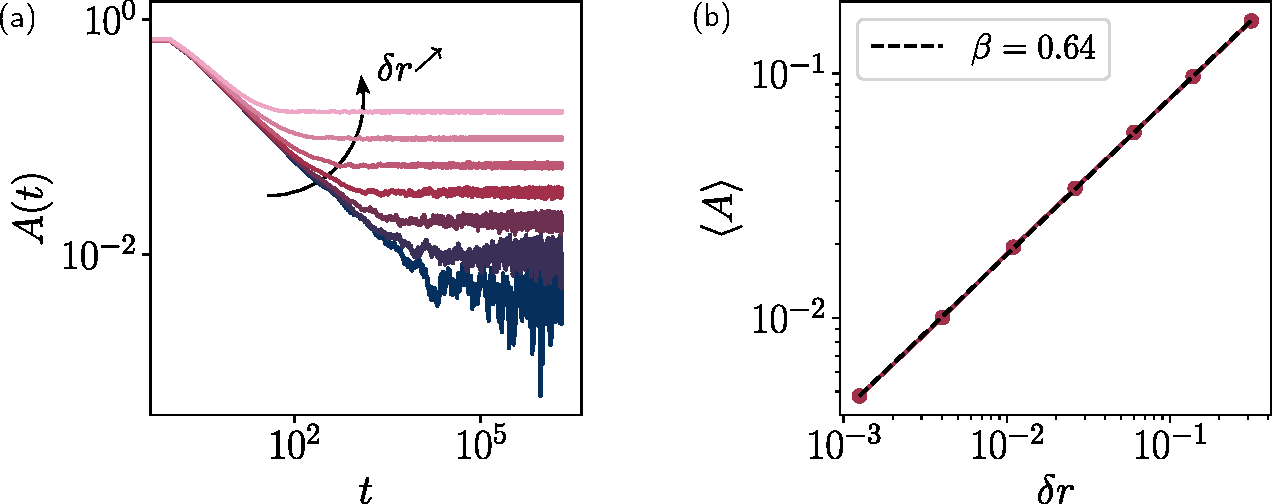
\includegraphics[width=0.9\textwidth]{Chapitre6/Figures/betaCDP_Langevin.pdf}
	\caption{Intégration numérique des équations de champs CDP. (a) Evolution de l'activité dans le système $ A $ en fonction du temps $t$ pour différentes distances au point critique $\delta r = \frac{r-r_c}{r_c}$. (b) Détermination de l'exposant $\beta$. Nous mesurons $r_c \approx -0.14418$ pour les valeurs de paramètres $\omega = 1$, $u = 1$, $\kappa = 0.25$, $\sigma = 1.4$ et une valeur moyenne du champ conservé $\bar{\sigma} = 1$.}
	\label{fig:TestDornicCDP}
\end{figure}

\subsection{Enjeux pratiques}

\subparagraph{}Dans cette sous-section, nous mettons en évidence les difficultés pratiques concernant l'établissement de telles théories de champ en prenant l'exemple représentatif de la transition vers l'écoulement.

\subparagraph{}Par équivalence avec la transition de dépiégeage, une théorie de champ intuitive pour la transition vers l'écoulement reviendrait à remplacer les termes en $\Delta A$ dans l'\autoref{eq:CDP2} par des convolutions avec le propagateur élastique de type Eshelby $\mathcal{G}\ast A$. Si cette formulation est en théorie valable pour l'équation sur la quantité conservée, elle pose un problème de principe dans le cas de l'équation sur l'activité. En effet, le propagateur associé présentant des parties négatives, cela signifie qu'une zone inactive caractérisée par $A = 0$ est susceptible de se voir attribuer une activité négative sous l'effet de cette interaction non-locale. Une solution intuitive à ce problème serait alors d'ajouter une partie locale à ce terme d'interaction afin qu'il prenne la forme $A\times \mathcal{G}\ast A$, assurant de ce fait que l'activité d'une zone inactive ne puisse pas être diminuée. Toutefois cela pose un second problème : dans ce cadre, une zone inactive ne peut pas être activée à distance (puisque le terme d'interaction à longue portée associé est nul), ce qui constitue un aspect essentiel du mécanisme que l'on cherche à modéliser.

\subparagraph{}La dynamique de bruit interne semblant devoir faire intervenir des interactions à longue portée de signes alternés (i.e. capables de favoriser comme de défavoriser la création d'activité), cette difficulté se retrouve dans toutes les théories intuitives que l'on peut proposer pour les différentes transitions. Les équations de champ que nous avons envisagées permettent donc toutes de répondre à ces deux critères :

\begin{itemize}
	\item faire intervenir des interactions capables de créer de l'activité dans des zones inactives à longue portée
	\item faire intervenir des interactions inhibitrices de l'activité à longue portée préservant la positivité de l'activité en tout point.
\end{itemize}

\subsection{Résultats préliminaires}

\subparagraph{}Dans cette section, nous présentons des théories que nous avons envisagé dans le cadre de la modélisation des transitions de réversibilité et d'écoulement. Les résultats préliminaires que nous avons obtenus montrent que les formulations intuitives des équations de champ pour modéliser les transitions convexes sont inadéquates. Plus particulièrement, nous montrons qu'avec des interactions associées à longue portée, celles-ci ne permettent pas de dépasser le paradigme $\beta \approx 1$. Afin de ne pas tomber dans l'écueil de présenter exhaustivement toutes nos tentatives non fructueuses, nous proposons dans cette sous-section de présenter simplement trois théories motivées par les modèles microscopiques que nous avons étudié dans cet ouvrage.

\paragraph{Exemple de théorie motivée par le modèle de Picard}

\subparagraph{}Dans le cadre de la modélisation continue du modèle de Picard, une théorie envisageable est celle représentée par les équations suivantes :

\begin{equation}
    \begin{aligned}
        \partial_t A (\mathbf{r}, t) &= \left(\omega \rho (\mathbf{r}, t)-r\right) A (\mathbf{r}, t) - uA^2 (\mathbf{r}, t) + \kappa \left(\mathcal{G}^+\ast A \right)(\mathbf{r}, t) + \kappa\left(\mathcal{G}\ast A \right)(\mathbf{r}, t)A (\mathbf{r}, t) \\
        &+\sigma \sqrt{A (\mathbf{r}, t)}\eta(\mathbf{r}, t)\\
        \partial_t \rho (\mathbf{r}, t) &= \kappa_\sigma \left(\mathcal{G}\ast A \right)(\mathbf{r}, t)
    \end{aligned}
\label{eq:YieldingD}
\end{equation}

\noindent avec $\mathcal{G}$ le porpagateur d'Eshelby et $\mathcal{G}^+$ sa partie positive définie selon :

\begin{equation}
	\mathcal{G}^+(\mathbf{r}) = \mathcal{G}(\mathbf{r})\Theta\left(\mathcal{G}(\mathbf{r})\right)
\end{equation}

\noindent avec $\Theta$ la fonction de Heaviside. Sous cette formulation, les deux critères énoncés précédemment sont respectés : le terme en $\sim \mathcal{G}^+\ast A$ permet une création à distance d'activité dans les zones inactives et le terme en $A\times \mathcal{G}\ast A$ permet une inhibition de l'activité à distance tout en préservant sa positivité.

\subparagraph{}En variant la valeur du paramètre $r$, l'intégration numérique de ces équations révèle bien la présence d'une transition de phase absorbante. Pour $r>r_c$, le système se stabilise à temps long dans un état stationnaire caractérisé par $\langle A \rangle > 0$ alors que pour $r<r_c$ il finit par tomber dans un état absorbant caractérisé par $A = 0$. Toutefois, en analysant l'évolution de l'activité en fonction de la distance au point critique $\delta r$, nous remarquons que cette transition semble caractérisée trivialement par $\beta \approx 1$, comme cela est illustré à la \autoref{fig:YieldingD}. D'après ces résultats préliminaires, cette formulation ne semble donc pas permettre de retranscrire la convexité de la transition et donc le processus de bruit interne inhérent à la dynamique modélisée.

\begin{figure}[h]
	\centering
	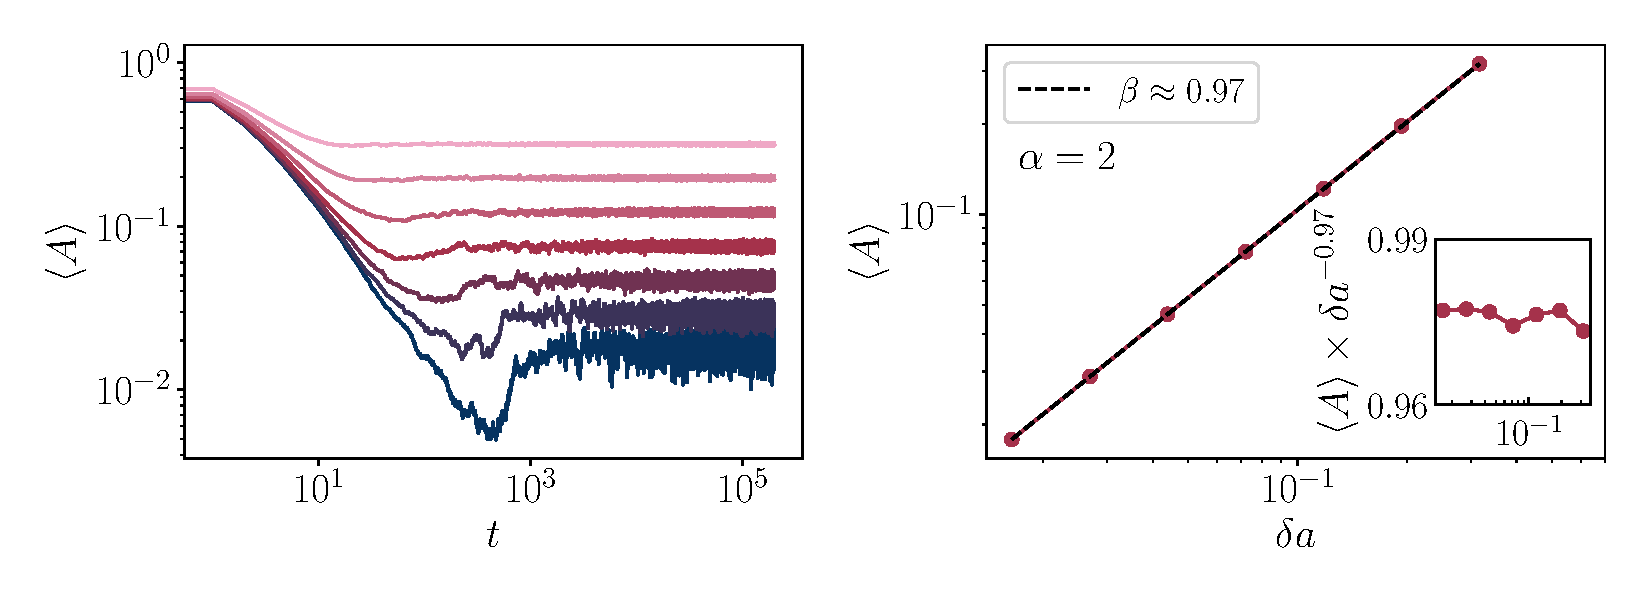
\includegraphics[width=\textwidth]{Chapitre5/Figures/YieldingD.pdf}
	\caption{Intégration numérique de l'\autoref{eq:YieldingD} dans un système 2D de taille $L=512$ avec comme valeur des paramètres : $\omega = 1$, $u = 1$, $\kappa = 0.25$, $\kappa_\sigma = 0.25$, $\sigma = 1$ et une valeur moyenne du champ conservé $\bar{\rho} = 1$. Le paramètre $r$ est varié dans l'ensemble $\{ 0.5214,  0.6153, 0.6726, 0.7076, 0.7290, 0.7420, 0.7500, 0.7549\}$. (a) Evolution de la valeur moyenne du champ d'activité en fonction du temps pour des différentes valeurs du paramètre $r$. (b) Evolution de la valeur moyenne de l'activité dans l'état stationnaire en fonction de la distance au point critique $\delta r$. Nous estimons ici $r_c \approx 0.7625$.}
	\label{fig:YieldingD}
\end{figure}

\paragraph{Exemple de théorie motivée par le modèle $\alpha$-ROM}

\subparagraph{}Dans l'étude menée par Mari et al. \cite{mari_absorbing_2022} sur le $0$-ROM, les auteurs ont proposé une théorie continue dérivée de celle de CDP en y introduisant un terme de création d'activité dû à la diffusion des particules passives. Dans le cadre d'interactions spatialisées comme nous avons considéré dans le cas du $\alpha$-ROM, cette théorie continue peut se généraliser simplement par la forme suivante (voir \autoref{sec:EqChampROM}) :

\begin{equation}
    \begin{aligned}
        \partial_t A (\mathbf{r}, t) &= \left(\omega \rho (\mathbf{r}, t)-r\right) A (\mathbf{r}, t) - uA^2 (\mathbf{r}, t) +\kappa \Delta A (\mathbf{r}, t)\\
        &+ \kappa \left(G\ast A \right)(\mathbf{r}, t)\left(1-\gamma \sqrt{ \left(G\ast A \right)(\mathbf{r}, t)}\right)\rho (\mathbf{r}, t)+ \sigma \sqrt{A (\mathbf{r}, t)}\eta (\mathbf{r}, t)\\
        \partial_t \rho (\mathbf{r}, t) &= \kappa_\sigma \Delta A (\mathbf{r}, t)
    \end{aligned}
\label{eq:SuspensionsB}
\end{equation}

\noindent avec $G(\mathbf{r})$ un propagateur positif décroissant comme $\sim 1/r^{2\alpha}$ à grande distance. En pratique, nous considérons le même propagateur que dans les modèles $\alpha$-ROM et conservons son implémentation décrite au \autoref{chapter:Susp}.

\subparagraph{}Afin de voir si cette formulation permet de reproduire la convexité de la transition, nous intégrons ces équations stochastiques pour différentes valeurs de $r$. Nous retrouvons alors une transition de phase absorbante dont la caractérisation préliminaire est présentée sur la \autoref{fig:SuspensionsB}. Via une analyse similaire au cas précédent, nous déterminons $\beta \approx 1.09$ pour $\alpha = 0.5$, la valeur $\beta = 1$ étant comprise dans les incertitudes de détermination. \`A cette valeur de la portée, nous sommes dans la limite de portée infinie du $\alpha$-ROM caractérisée précédemment par $\beta \approx 1.85$. Ce résultat $\beta \approx 1$ suggère donc que cette théorie continue ne permet pas non plus d'expliquer la convexité de la transition dans le modèle de particules.

\begin{figure}[h]
	\centering
	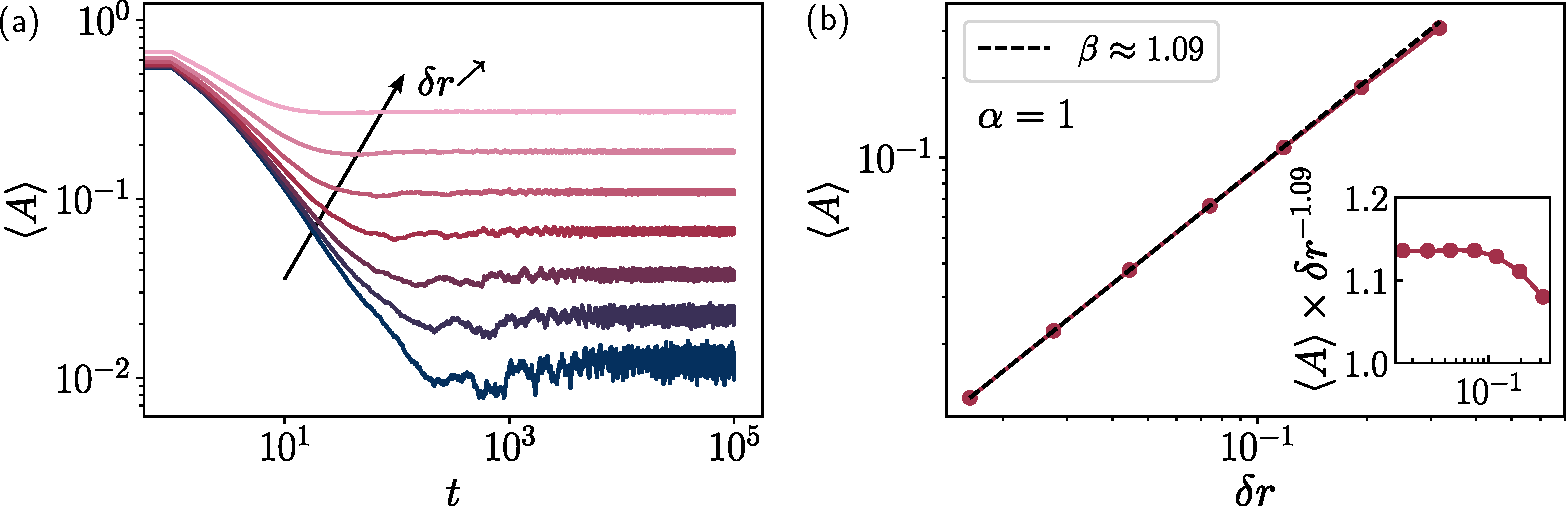
\includegraphics[width=\textwidth]{Chapitre5/Figures/SuspensionsB.pdf}
	\caption{Intégration numérique de l'\autoref{eq:SuspensionsB} dans un système 2D de taille $L=1024$ avec comme valeur des paramètres : $\omega = 0.04$, $u = 1$, $\kappa = 0.25$, $\kappa_\sigma = 0.01$, $\sigma = 1$, $\gamma = 0.1$ et une valeur moyenne du champ conservé $\bar{\rho} = 25$. Le paramètre $r$ est varié dans l'ensemble $\{ 0.602, 0.711, 0.777, 0.816, 0.842, 0.857, 0.867, 0.872\}$. (a) Evolution de la valeur moyenne du champ d'activité en fonction du temps pour des différentes valeurs du paramètre $r$. (b) Evolution de la valeur moyenne de l'activité dans l'état stationnaire en fonction de la distance au point critique $\delta r$. Nous estimons ici $r_c \approx 0.8813$.}
	\label{fig:SuspensionsB}
\end{figure}

\paragraph{Approche naïve via l'attendu champ moyen}

\label{sec:CMnaif}

\subparagraph{}Face aux difficultés posées par la prise en compte d'interactions à longue portée non-monotones, nous pouvons imaginer une autre voie vers la convexité via la modification des termes locaux de la théorie de champ CDP. C'est notamment l'idée déjà proposée par Mari et al. \cite{mari_absorbing_2022} qui considère les équations de champ suivantes dans le cas d'une portée d'interaction infinie :

\begin{equation}
\begin{aligned}
	&\partial_t A(\mathbf{r}, t) = (\omega\rho (\mathbf{r}, t) - r)A(\mathbf{r}, t) - uA^{3/2}(\mathbf{r}, t) + \kappa\Delta A (\mathbf{r}, t) + \sigma \sqrt{A(\mathbf{r}, t)} \eta(\mathbf{r}, t)\\
	&\partial_t \rho (\mathbf{r}, t) = \kappa\Delta A (\mathbf{r}, t)
\end{aligned}
\label{eq:CDP32}
\end{equation}

\noindent Dans une approche habituelle de la théorie de champ moyen qui équivaut à négliger les termes de bruit et d'interaction, cette théorie amène en effet à un exposant $\beta^\text{MF} = 2$.

\subparagraph{}Pour comprendre si cette formulation permet effectivement de retrouver une transition convexe caractérisée par $\beta > 1$, nous intégrons l'\autoref{eq:CDP32} dans sa forme champ moyen. Pour ce faire, le terme d'interaction local $\Delta A$ est remplacé par $\bar{A}-A$ avec $\bar{A}$ la valeur moyenne instantanée du champ d'activation. Toujours en faisant varier le paramètre $r$, nous observons une transition de phase absorbante mais dont la criticalité semble être encore caractérisée par $\beta \approx 1$, comme nous le représentons à la \autoref{fig:MFCDP32}. Bien que ces résultats restent préliminaires, cette étude présente une approche du point critique raisonnable qui suggère que la transition n'est effectivement pas convexe dans la limite de très longue portée.

\subparagraph{}Même si cela peut apparaître surprenant, dans la partie suivante, nous montrons que ce résultat est en fait prévisible d'un point de vue analytique. Comme des études précédentes l'ont montré, les théories de champ faisant intervenir des bruits multiplicatifs ne possèdent pas des propriétés champ moyen dérivables trivialement \cite{munoz_mean_field_2005, munoz_multiplicative_2003}. \`A la place, un autre traitement du champ moyen doit être opéré. Celui-ci mène alors à un exposant $\beta^\text{MF} = 1$ quel que soit le degré de non-linéarité choisi dans une théorie présentant un terme de bruit multiplicatif en $\sim \sqrt{A(\mathbf{r}, t)}$.

\begin{figure}[h]
	\centering
	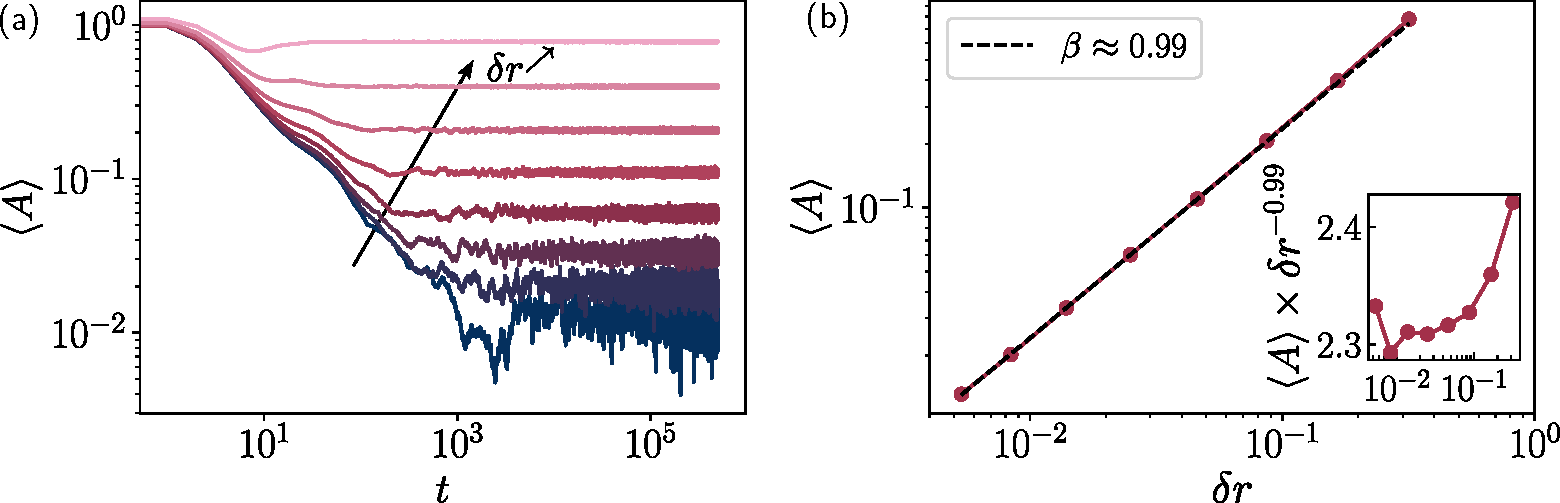
\includegraphics[width=\textwidth]{Chapitre5/Figures/MFCDP32.pdf}
	\caption{Intégration numérique de l'\autoref{eq:CDP32} dans un système 2D de taille $L=1024$ avec comme valeur des paramètres : $\omega = 1$, $u = 0.5$, $\kappa = 0.25$, $\kappa_\sigma = 0.01$, $\sigma = 1$, $\gamma = 0.1$ et une valeur moyenne du champ conservé $\bar{\rho} = 1$. Le paramètre $r$ est varié dans l'ensemble $\{ 0.2462, 0.3010, 0.3295, 0.3442, 0.3518, 0.3558, 0.3578, 0.3589\}$. (a) Evolution de la valeur moyenne du champ d'activité en fonction du temps pour des différentes valeurs du paramètre $r$. (b) Evolution de la valeur moyenne de l'activité dans l'état stationnaire en fonction de la distance au point critique $\delta r$. Nous estimons ici $r_c \approx 0.36083$.}
	\label{fig:MFCDP32}
\end{figure}

\subsection{Approches champ moyen des transitions avec bruit multiplicatif}

\subparagraph{}Dans cette partie, nous expliquons pourquoi les théories de champ faisant intervenir un bruit multiplicatif ne peuvent pas être associées à un comportement champ moyen via la méthode habituelle. D'habitude, pour déterminer l'exposant $\beta$ dans la limite champ moyen, il est d'usage de simplifier les équations de champs associées en supprimant les termes de dépendances spatiales et de bruit. Si l'on prend l'exemple de la théorie DP, celle-ci devient dans ce cas (voir \autoref{eq:eqDP}) :

\begin{equation}
	\frac{\mathrm{d}A}{\mathrm{d}t} = rA(t) - u A^2(t)
\end{equation}

\noindent dont on tire de la solution stationnaire $\beta = 1$.

\paragraph{Principe de l'approche}

\subparagraph{}Dans le cadre général d'une équation de champ représentée par un bruit multiplicatif, cette méthode ne tient plus, comme l'ont montré les travaux de Munoz et al. \cite{munoz_multiplicative_2003, munoz_multiplicative_2003}. Dans ces études, les auteurs se sont concentrés sur la théorie de champ suivante :

\begin{equation}
	\partial_t A(\mathbf{r}, t) = rA(\mathbf{r}, t) - uA^{p+1}(\mathbf{r}, t) + \kappa\nabla^2 A (\mathbf{r}, t) + \sigma A(\mathbf{r}, t) \eta(\mathbf{r}, t)
	\label{eq:eqMN}
\end{equation}

\noindent représentant la classe \textit{multiplicative noise} (MN). Au lieu de déterminer l'exposant $\beta$ via la méthode habituelle qui ne permettait l'accord avec les résultats numériques, Munoz et al. ont proposé de rendre cette équation 0-dimensionnelle en considérant un système discret de $N$ sites dans la limite de couplage total. Dans ce cas, l'opérateur laplacien pour un site $i$ devient :

\begin{equation}
    \nabla^2 A_i = \frac{1}{N-1}\sum_{j\neq i}\left( A_j - A_i \right) = \mathcal{A} - A_i
\end{equation}

\noindent avec $\mathcal{A}$ la valeur moyenne de l'activité. Dans la limite de couplage total où tous le sites sont équivalents, on a donc, en abandonnant la notation indicielle :

\begin{equation}
	\partial_t A = (r-\kappa)A - uA^{p+1} + \kappa\mathcal{A} + \sigma A \eta
	\label{eq:eqMN0}
\end{equation}

\subparagraph{}Nous pouvons alors associer à cette équation de Langevin une équation de Fokker-Planck stationnaire au sens de Ito :

\begin{equation}
    0 = -\partial_A\left( \left[(r-\kappa)A - b\phi^{p+1}+\kappa\mathcal{A} \right] P(A)\right) + \frac{\sigma^2}{2}\partial_A^2\left( A^2 P(A)\right)
\end{equation}

\noindent dont on peut dériver la solution analytique :

\begin{equation}
    P(A) = A^{-2-2(\kappa-r)/\sigma^2}\exp\left( -\frac{2u}{p\sigma^2}A^p - \frac{2\mathcal{A} \kappa}{\sigma^2}\frac{1}{A} \right)
\end{equation}

\subparagraph{}Afin de déterminer le comportement critique associé à l'\autoref{eq:eqMN0}, il suffit alors de développer la relation d'auto-cohérence :

\begin{equation}
    \mathcal{A} = \langle A \rangle = \frac{\int_0^\infty\mathrm{d}A~\phi P(A)}{\int_0^\infty\mathrm{d}A~P(A)}
\end{equation}

\noindent pour déterminer l'exposant $\beta$ tel que $\langle A \rangle \sim r^\beta$. Le calcul développé dans \cite{munoz_multiplicative_2003, munoz_multiplicative_2003} amènent alors à :

\begin{equation}
	\beta = \mathrm{max}\left\{ \frac{1}{p}, \frac{\sigma^2}{2\kappa}\right\}
\end{equation}

\noindent qui ne permet de retrouver la prédiction naïve $\beta = 1/p$ que dans un régime de faible bruit $\sigma^2 < 2\kappa/p$.

\paragraph{Application au cas de la théorie DP généralisée}

\subparagraph{}Dans cette partie, nous proposons de suivre cette approche dans le cas des équations de champ associées à la classe DP avec un degré de non-linéarité arbitraire, i.e. avec un terme de bruit en $\sim \sqrt{A}$ et non en $\sim A$ comme dans le cas de la classe MN :

\begin{equation}
	\partial_t A(\mathbf{r}, t) = rA(\mathbf{r}, t) - uA^{p+1}(\mathbf{r}, t) + \kappa\nabla^2 A (\mathbf{r}, t) + \sigma \sqrt{A(\mathbf{r}, t)} \eta(\mathbf{r}, t)
	\label{eq:eqDParb}
\end{equation}

\noindent En suivant le même raisonnement, nous obtenons la distribution stationnaire de l'activité :

\begin{equation}
    P(A)=A^{-1+2\kappa\mathcal{A}/\sigma^2}\exp\left( \frac{2(r-\kappa)}{\sigma^2}A-\frac{2u}{(p+1)\sigma^2}A^{p+1} \right)
\end{equation}

\noindent et la relation d'auto-cohérence :

\begin{equation}
    \mathcal{A} = \frac{\int_ 0^\infty \mathrm{d}A~A^{2\kappa\mathcal{A}/\sigma^2}\exp\left( -2\frac{(\kappa-r)}{\sigma^2} A - \frac{2u}{(p+1)\sigma^2}A^{p+1} \right)}{\int_ 0^\infty \mathrm{d}A~A^{-1+2\kappa\mathcal{A}/\sigma^2}\exp\left( -2\frac{(\kappa-r)}{\sigma^2} A - \frac{2u}{(p+1)\sigma^2}A^{p+1} \right)}
\end{equation}

\subparagraph{}La difficulté réside dans le fait que le dénominateur du membre de droite diverge. Toutefois, en menant une intégration par partie nous pouvons obtenir la relation suivante :

\begin{equation}
    \frac{f\left( \mathcal{A} + p\sigma^2/2\kappa, r \right)}{f\left(\mathcal{A}, r\right)}=\frac{r}{u},\quad f(\mathcal{A}, r) = \int_ 0^\infty \mathrm{d}A~A^{2\kappa\mathcal{A}/\sigma^2}\exp\left( -2\frac{(\kappa-r)}{\sigma^2} A - \frac{2u}{(p+1)\sigma^2}A^{p+1} \right)
    \label{eq:selfconsistencyDP}
\end{equation}

\noindent qui est a priori cette fois bien définie. Nous définisson alors le paramètre critique $r_c$ selon la relation :

\begin{equation}
    r_c = u\frac{f\left(p\sigma^2/2\kappa, r_c \right)}{f\left(0, r_c\right)}
\end{equation}

\noindent En considérant que la fonction $f$ se comporte bien, on peut la développer en série pour obtenir : 

\begin{equation}
    \mathcal{A} = \frac{1-r_c\left( \frac{\partial_r f(\frac{p\sigma^2}{2\kappa},r_c)}{f(\frac{p\sigma^2}{2\kappa},r_c)}- \frac{\partial_rf(0,r_c)}{f(0,r_c)} \right)}{r_c\left( \frac{\partial_\mathcal{A} f(\frac{p\sigma^2}{2\kappa},r_c)}{f(\frac{p\sigma^2}{2\kappa},r_c)}- \frac{\partial_\mathcal{A} f(0,r_c)}{f(0,r_c)} \right)}\epsilon,\quad \epsilon = \frac{r-r_c}{r_c}
\end{equation}

\noindent ce qui suggère que l'on a $\beta^\text{CM} = 1$ peu importe le degré de non-linéarité $p$ de l'équation de champ.

\paragraph{Résolution numérique}

\subparagraph{}Pour contrôler nos calculs et les hypothèses faites, nous résolvons numériquement l'équation d'auto-cohérence \autoref{eq:selfconsistencyDP} pour obtenir $\mathcal{A} = f(r)$ avec le logiciel Mathematica. Sur la figure \autoref{fig:MathematicaMunoz} nous présentons les résultats obtenus pour la détermination de l'exposant $\beta$ pour différents degrés de non-linéarité $p$. Comme nous pouvons le remarquer, la mesure $\beta^\text{CM}=1$ semble être retrouvée peu importe la valeur de $p$.

\begin{figure}[h]
	\centering
	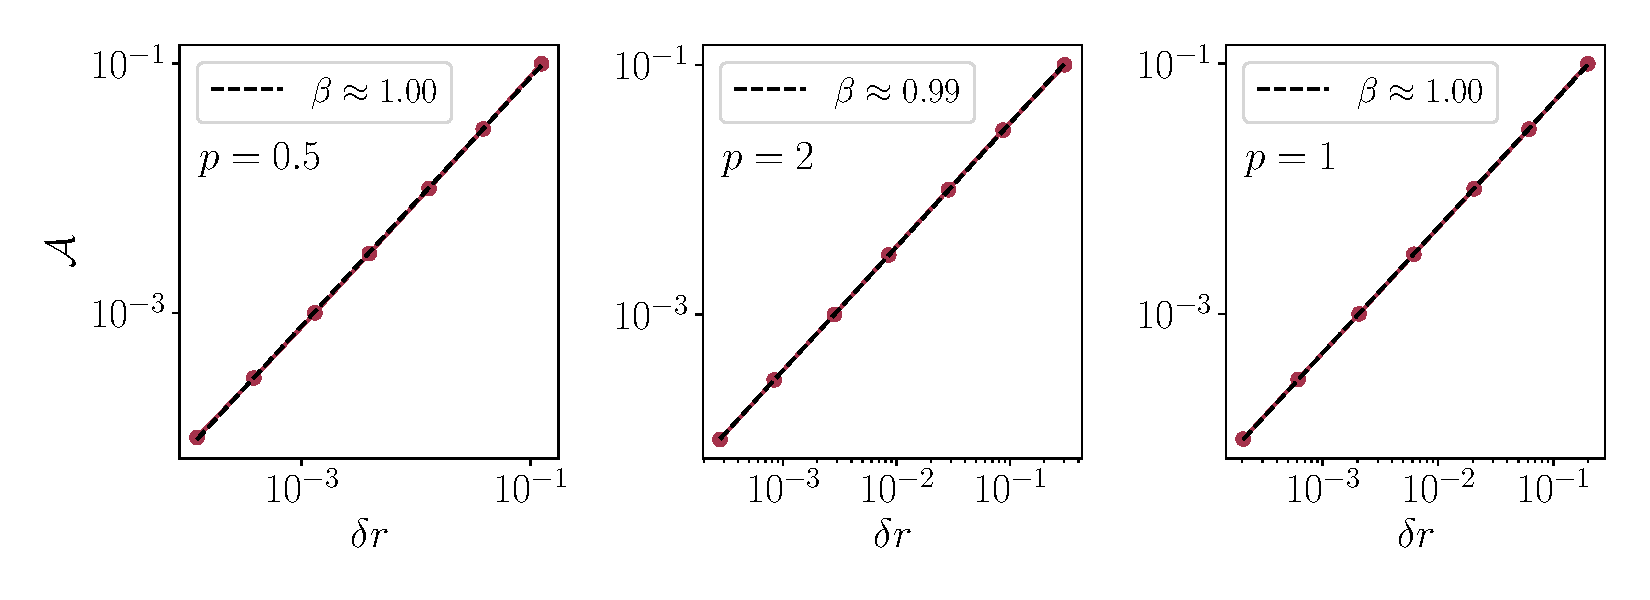
\includegraphics[width=\textwidth]{Chapitre6/Figures/MathematicaMunozDP.pdf}
	\caption{Détermination de l'exposant $\beta$ via la résolution numérique de l'\autoref{eq:selfconsistencyDP} pour différentes valeurs du degré de non-linéarité $p$.}
	\label{fig:MathematicaMunoz}
\end{figure}

\subparagraph{}Ainsi, ce raisonnement, peut-être discutable, semble montrer qu'en effet, le degré de non-linéarité dans l'équation de champ ne permet pas de modifier la valeur de l'exposant $\beta$ dans la limite de champ moyen. Cela permet de proposer une explication aux résultats suprenant de la \autoref{sec:CMnaif}.

\subsection{Conclusion de la section}

\subparagraph{}En conclusion, il ne semble pas aisé de mettre en évidence des équations de champ permettant de produire une transition de phase absorbante convexe. Que ce soit via l'introduction d'interactions à longue portée de signe alterné, l'introduction d'une non-analyticité dans le terme non-local ou la modification du degré de non-linéarité du terme non-linéaire local, le comportement critique dans la limite de longue portée semble être toujours limité à $\beta = 1$. Les tests d'intégration que nous avons présenté ici sont les représentants de nombreux autres essais pointant vers le même résultat. 

\subparagraph{}Ces difficultés suggèrent que le cadre représenté par les équations de type CDP/LR-CDP n'est pas le bon point de départ. Pour poursuivre dans cette direction, il faudrait donc considérer des modifications plus profondes de ces théories afin d'appréhender plus justement le mécanisme de diffusion vers un bord absorbant, qui est l'élément central de ces transitions. Nous pourrions imaginer que cette modélisation passe par la considération d'une nouvelle forme de bruit non-locale, celle d'une dynamique d'un champ complémentaire représentant la distance au bord absorbant ou encore celle d'une complexification de l'équation sur la dynamique du champ conservé. Notons par ailleurs que la modification de la forme du bruit dans l'équation sur l'activité ou l'ajout d'un bruit dans la dynamique du champ conservé ne sont pas des éléments directs à implémenter et nécessitent la modification de tout notre schéma numérique. Une telle investigation gagnerait donc à être sérieusement motivée par des arguments émergents des dynamiques microscopiques.

\subparagraph{}La différence de formulation entre ces théories de champs et les modèle à la Hébraud-Lequeux pourrait être un indice de ces potentielles profondes modifications. Une autre piste d'ouverture pourrait donc être d'essayer de réaliser une équivalence entre ces modèles et une équation de champ triviale dans la limite de champ moyen. \`A ce stade de notre recherche, nous n'avons toutefois pas encore pu explorer cette pistes de manière pertinente.

